\documentclass[a4paper,12pt]{report}

\usepackage{alltt, fancyvrb, url}
\usepackage{graphicx}
\usepackage[utf8]{inputenc}
\usepackage{float}
\usepackage{xcolor}
\usepackage{hyperref}
\usepackage[italian]{datetime2}

% Questo commentalo se vuoi scrivere in inglese.
\usepackage[italian]{babel}

\usepackage[italian]{cleveref}

\title{Relazione progetto per\\``Gioco dell'Oca``}

\author{Nicolae Balaban\\ Antonino Cardillo}
\date{\DTMdate{2026-10-01}}


\begin{document}

\maketitle

\tableofcontents

\chapter{Analisi}

\section{Descrizione e requisiti}

Il software si propone di realizzare una versione digitale in chiave moderna del classico gioco da tavolo "\textbf{Gioco dell'Oca}". L'obiettivo è quello di fornire un'esperienza interattiva pensata per un gruppo che va da 2 a 4 partecipanti, mantenendo lo spirito ludico e la natura di competizione basata sulla casualità tipica del gioco originale. All'avvio, l'applicazione deve permettere all'utente di navigare tramite un menu principale per avviare una nuova partita, modificare le impostazioni, consultare le regole o uscire dal gioco. Prima dell'inizio di una partita, i giocatori devono potersi registrare inserendo il proprio nickname e scegliendo una pedina identificativa. Il gioco si svolge a turni su un percorso predefinito composto da un numero finito di caselle. L'avanzamento dei giocatori è determinato dal lancio di 1/2 dado/i virtuale a 6 facce. Lungo il percorso sono dislocate caselle speciali che alterano il normale svolgimento della partita, offrendo vantaggi (bonus), svantaggi (malus) o bloccando temporaneamente il giocatore (prigione). La partita si conclude quando un giocatore raggiunge l'esatta posizione dell'ultima casella del percorso.


\subsubsection{Requisiti funzionali}
\begin{itemize}
	\item \textbf{Menu Principale:} L'applicazione deve fornire un menu con le opzioni: "Nuova partita", "Impostazioni", "Regole", "Esci".
	\item \textbf{Configurazione Partita:} Il sistema deve permettere la selezione del numero di partecipanti (da 2 a 4). Per ciascun giocatore deve essere possibile inserire un nickname e selezionare una pedina associata.
	\item \textbf{Svolgimento a Turni:} I giocatori si alternano secondo un ordine predefinito. Durante il proprio turno, un giocatore lancia i dadi a 6 facce per muovere la propria pedina di un numero corrispondente di posizioni sul tabellone.
    \item \textbf{Tipi di Caselle:} Il percorso è composto da:
    \begin{itemize}
        \item Casella Normale: non applica alcun effetto aggiuntivo; indica la posizione sul tabellone.
        \item Casella Speciale: applica istantaneamente un effetto bonus (es. avanzare ulteriormente) o malus (es. retrocedere) al giocatore che vi capita sopra.
        \item Casella Prigione: situata a metà esatta del percorso, blocca il giocatore per un intero turno prima di potersi muovere nuovamente.
    \end{itemize}
    \item \textbf{Condizione di Vittoria:} Il sistema deve decretare la fine della partita e proclamare il vincitore non appena un giocatore raggiunge esattamente l'ultima casella del percorso. Qualora il risultato del dado porti il giocatore oltre l'ultima casella, la pedina "rimbalza" indietro del numero di posizioni eccedenti, senza vincere la partita.
    \item \textbf{Sistema Audio (opzionale):} Il gioco deve riprodurre effetti sonori specifici (es. per il lancio del dado e l'attivazione di caselle speciali) e una traccia musicale di sottofondo il cui volume sia configurabile nelle impostazioni.
\end{itemize}

\subsubsection{Requisiti non funzionali}
\begin{itemize}
	\item \textbf{Modularità ed Estensibilità:} Il software deve essere manutenibile ed estendibile, in modo da poter accogliere nuove regole di gioco con un impatto limitato sulle componenti esistenti.
    \item \textbf{Reattività e Sincronizzazione:} L'interfaccia grafica deve riflettere in maniera istantanea e continua i cambiamenti dello stato della partita. Ogni azione (come il lancio del dado o l'applicazione di un effetto) deve mostrare le animazioni e gli aggiornamenti visivi pertinenti senza latenze percepibili.
    \item \textbf{Integrità dei Dati:} Il sistema deve mantenere lo stato interno in maniera sempre coerente, rendendo impossibile l'insorgere di posizioni illegali sul tabellone, turni eseguiti fuori sequenza o dati discordanti tra giocatori.
    \item \textbf{Portabilità:} Il software deve essere in grado di essere eseguito indipendentemente dal sistema operativo sottostante.
\end{itemize}


\section{Modello del Dominio}

Il dominio del problema ruota attorno al concetto di \texttt{Partita}, che rappresenta la singola istanza del gioco e aggrega le entità principali necessarie al suo svolgimento. A una partita partecipano molteplici entità \texttt{Giocatore}, ognuna identificata da informazioni anagrafiche (nickname) e rappresentata visivamente sul percorso da una Pedina.

La partita si svolge interamente su un \texttt{Tabellone}, il quale è logicamente strutturato come una sequenza ordinata di elementi \texttt{Casella}. L'entità casella definisce il percorso e si specializza in tre forme distinte in base al comportamento richiesto: la \texttt{CasellaNormale}, la \texttt{CasellaSpeciale} (che racchiude la logica per l'assegnazione di un bonus o un malus sul posizionamento), e la \texttt{CasellaPrigione}, un vincolo specifico di blocco del turno. La progressione sul tabellone è unicamente demandata all'entità \texttt{Dado}, incaricata di fornire un valore discreto per il calcolo del movimento. Tutte queste entità interagiscono per definire lo stato di avanzamento.

\begin{figure}[H]
	\centering{}
	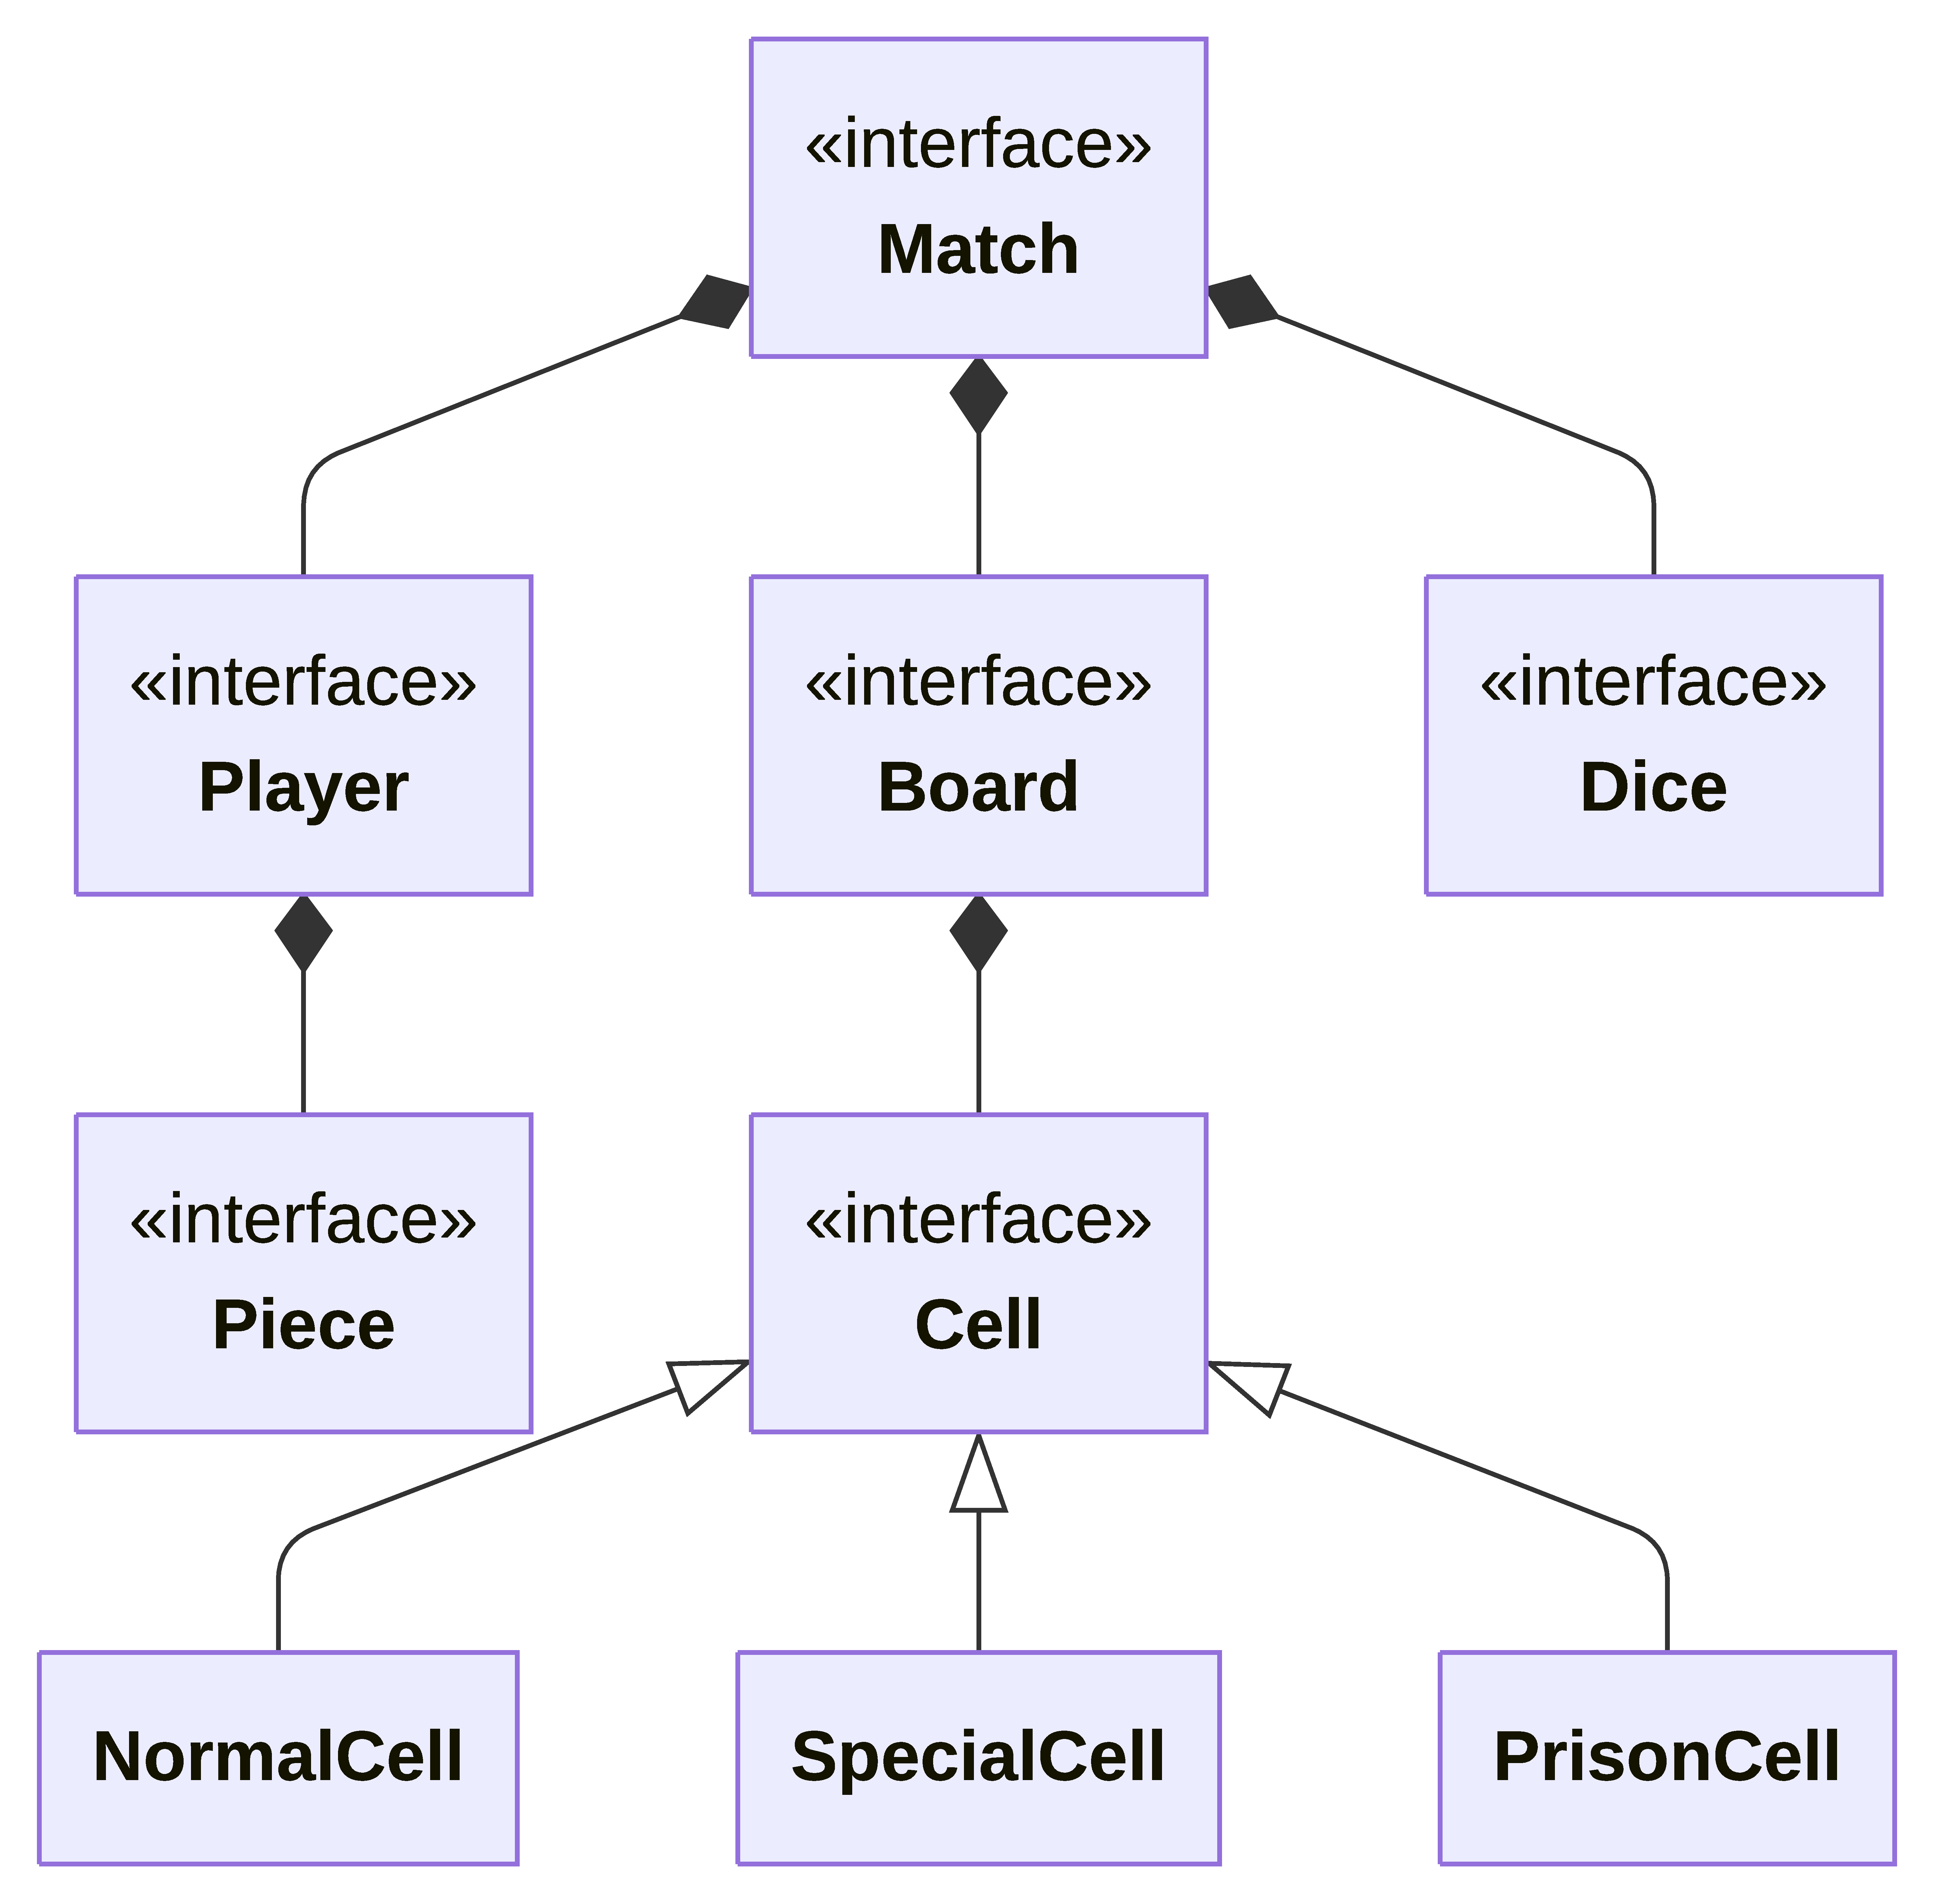
\includegraphics[width=\textwidth]{img/Figura1.1.pdf}
	\caption{Schema UML dell'analisi del dominio, con rappresentate le entità principali ed i rapporti fra loro.}
	\label{img:analysis}
\end{figure}

\chapter{Design}

\section{Architettura}

L'architettura del sistema adotta il pattern Model-View-Controller (MVC), scelto per separare in modo netto la logica di gioco, la gestione dello stato della partita e la sua presentazione all'utente.\\
\\
Il \textbf{Model} coincide con il dominio applicativo descritto nel capitolo precedente: la Partita e le entità ad essa collegate (Tabellone, Giocatore, Casella, Dado) mantengono lo stato della partita ed espongono le operazioni necessarie per modificarlo, senza avere alcuna conoscenza di come tali informazioni verranno successivamente presentate.\\
\\
Il \textbf{Controller}, è il punto di ingresso per le azioni provenienti dall'utente: avvia una nuova partita, gestisce l'alternanza dei turni, inoltra al Model le richieste conseguenti alle azioni del giocatore (ad esempio il lancio del dado) e verifica le condizioni di vittoria al termine di ogni turno.\\
\\
La \textbf{View} si occupa unicamente di mostrare il gioco a schermo (menu, tabellone, animazioni) e di raccogliere le azioni dell'utente, come il click per tirare il dado. Non ha alcun riferimento diretto al Model e non lo osserva: è il Controller che, dopo aver modificato lo stato del Model, invoca esplicitamente i metodi della View (ad esempio \texttt{showDiceResult(...)}, \texttt{showCurrentTurn(...)}, \texttt{updatePlayerPositions(...)}) per aggiornare l'interfaccia. La View inoltra le azioni dell'utente al Controller tramite \\callback (ad esempio \texttt{controller.rollDice())}.\\
\\

Grazie a questa divisione, sostituire in blocco la View (ad esempio per passare a una libreria grafica diversa) non causerebbe alcuna modifica nel Model. Ogni schermata dell'applicazione è organizzata in una coppia Controller–View dedicata (ad esempio \texttt{MatchController}/\texttt{MatchView},\\ \texttt{SettingsController}/\texttt{SettingsView}, ecc.): ciascun Controller dipende esclusivamente dall'interfaccia della propria View, mai dall'implementazione concreta.


\begin{figure}[h]
\centering{}
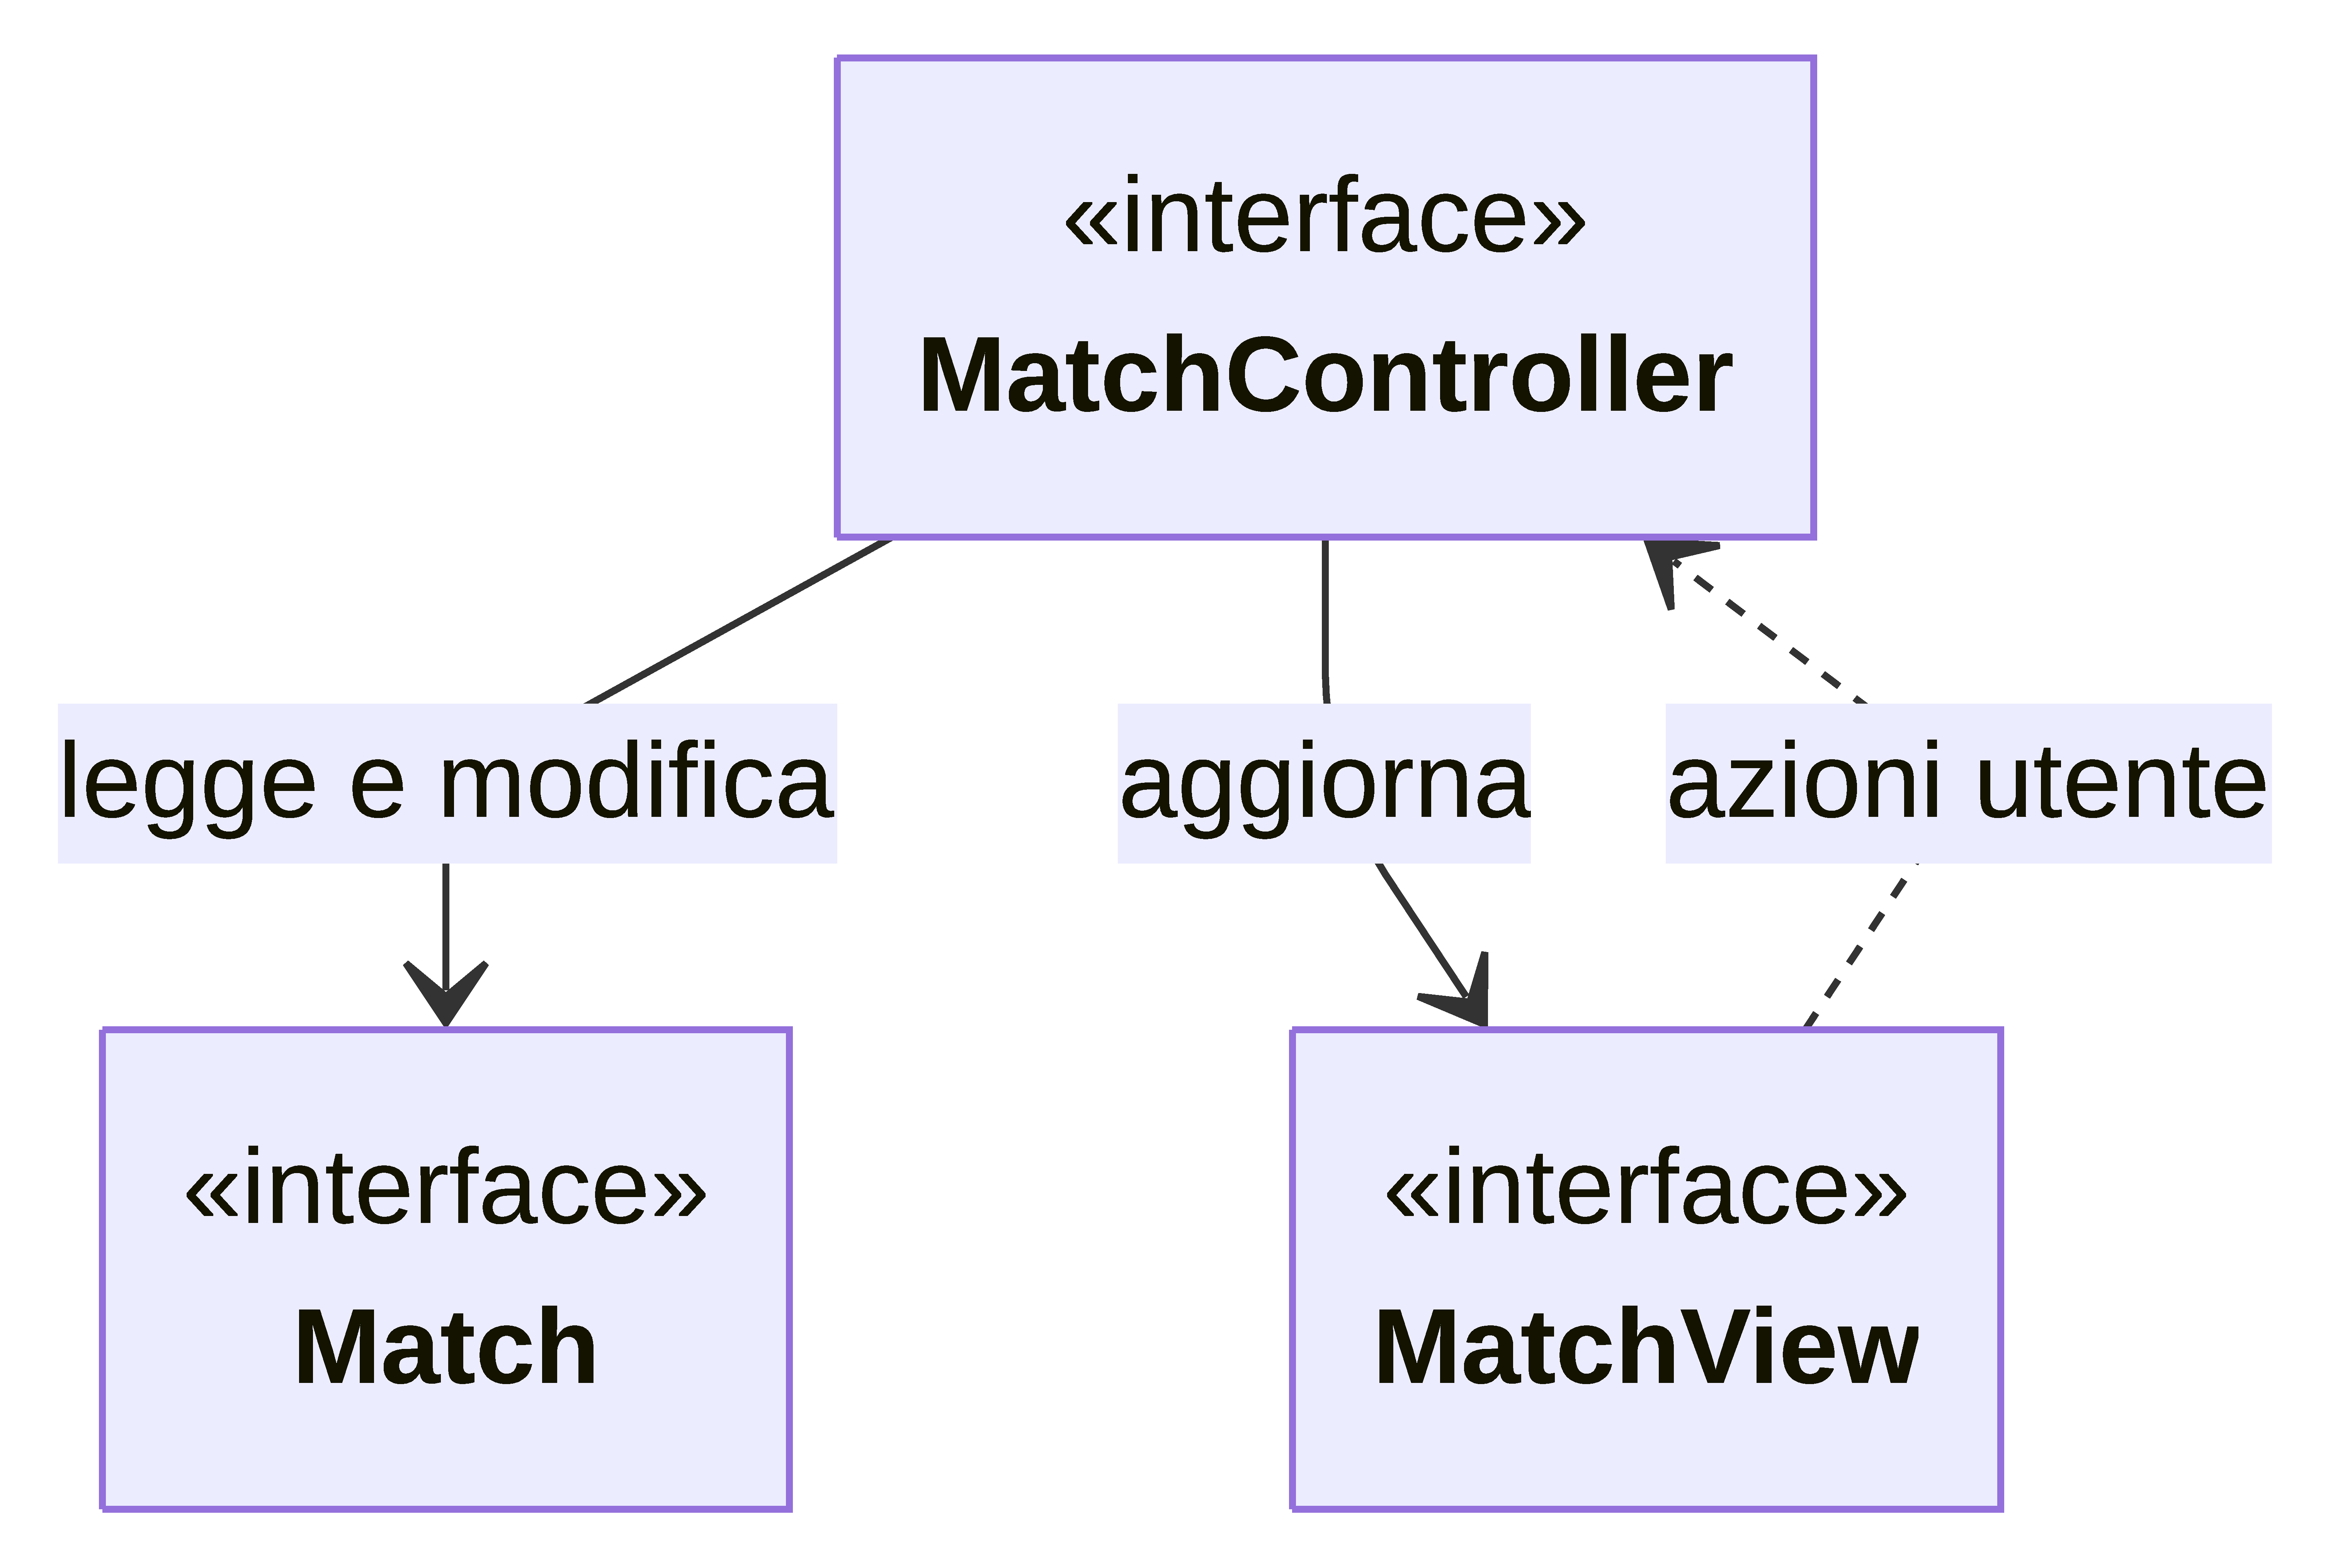
\includegraphics[width=\textwidth]{img/Figura2.1.pdf}
\caption{Schema UML architetturale MVC, esemplificato sulla partita. Il \texttt{MatchController} legge e modifica lo stato del \texttt{Match} (Model), poi aggiorna la \texttt{MatchView} invocandone i metodi. La View non ha alcuna dipendenza dal Model: inoltra le azioni dell'utente al Controller. Lo stesso schema si ripete per ogni coppia Controller–View dell'applicazione.}
\label{}
\end{figure}




\section{Design dettagliato}
\subsection{Nicolae Balaban}
\subsubsection{Architettura di navigazione e disaccoppiamento dei Controller (Application Controller)}

\begin{figure}[H]
\centering{}
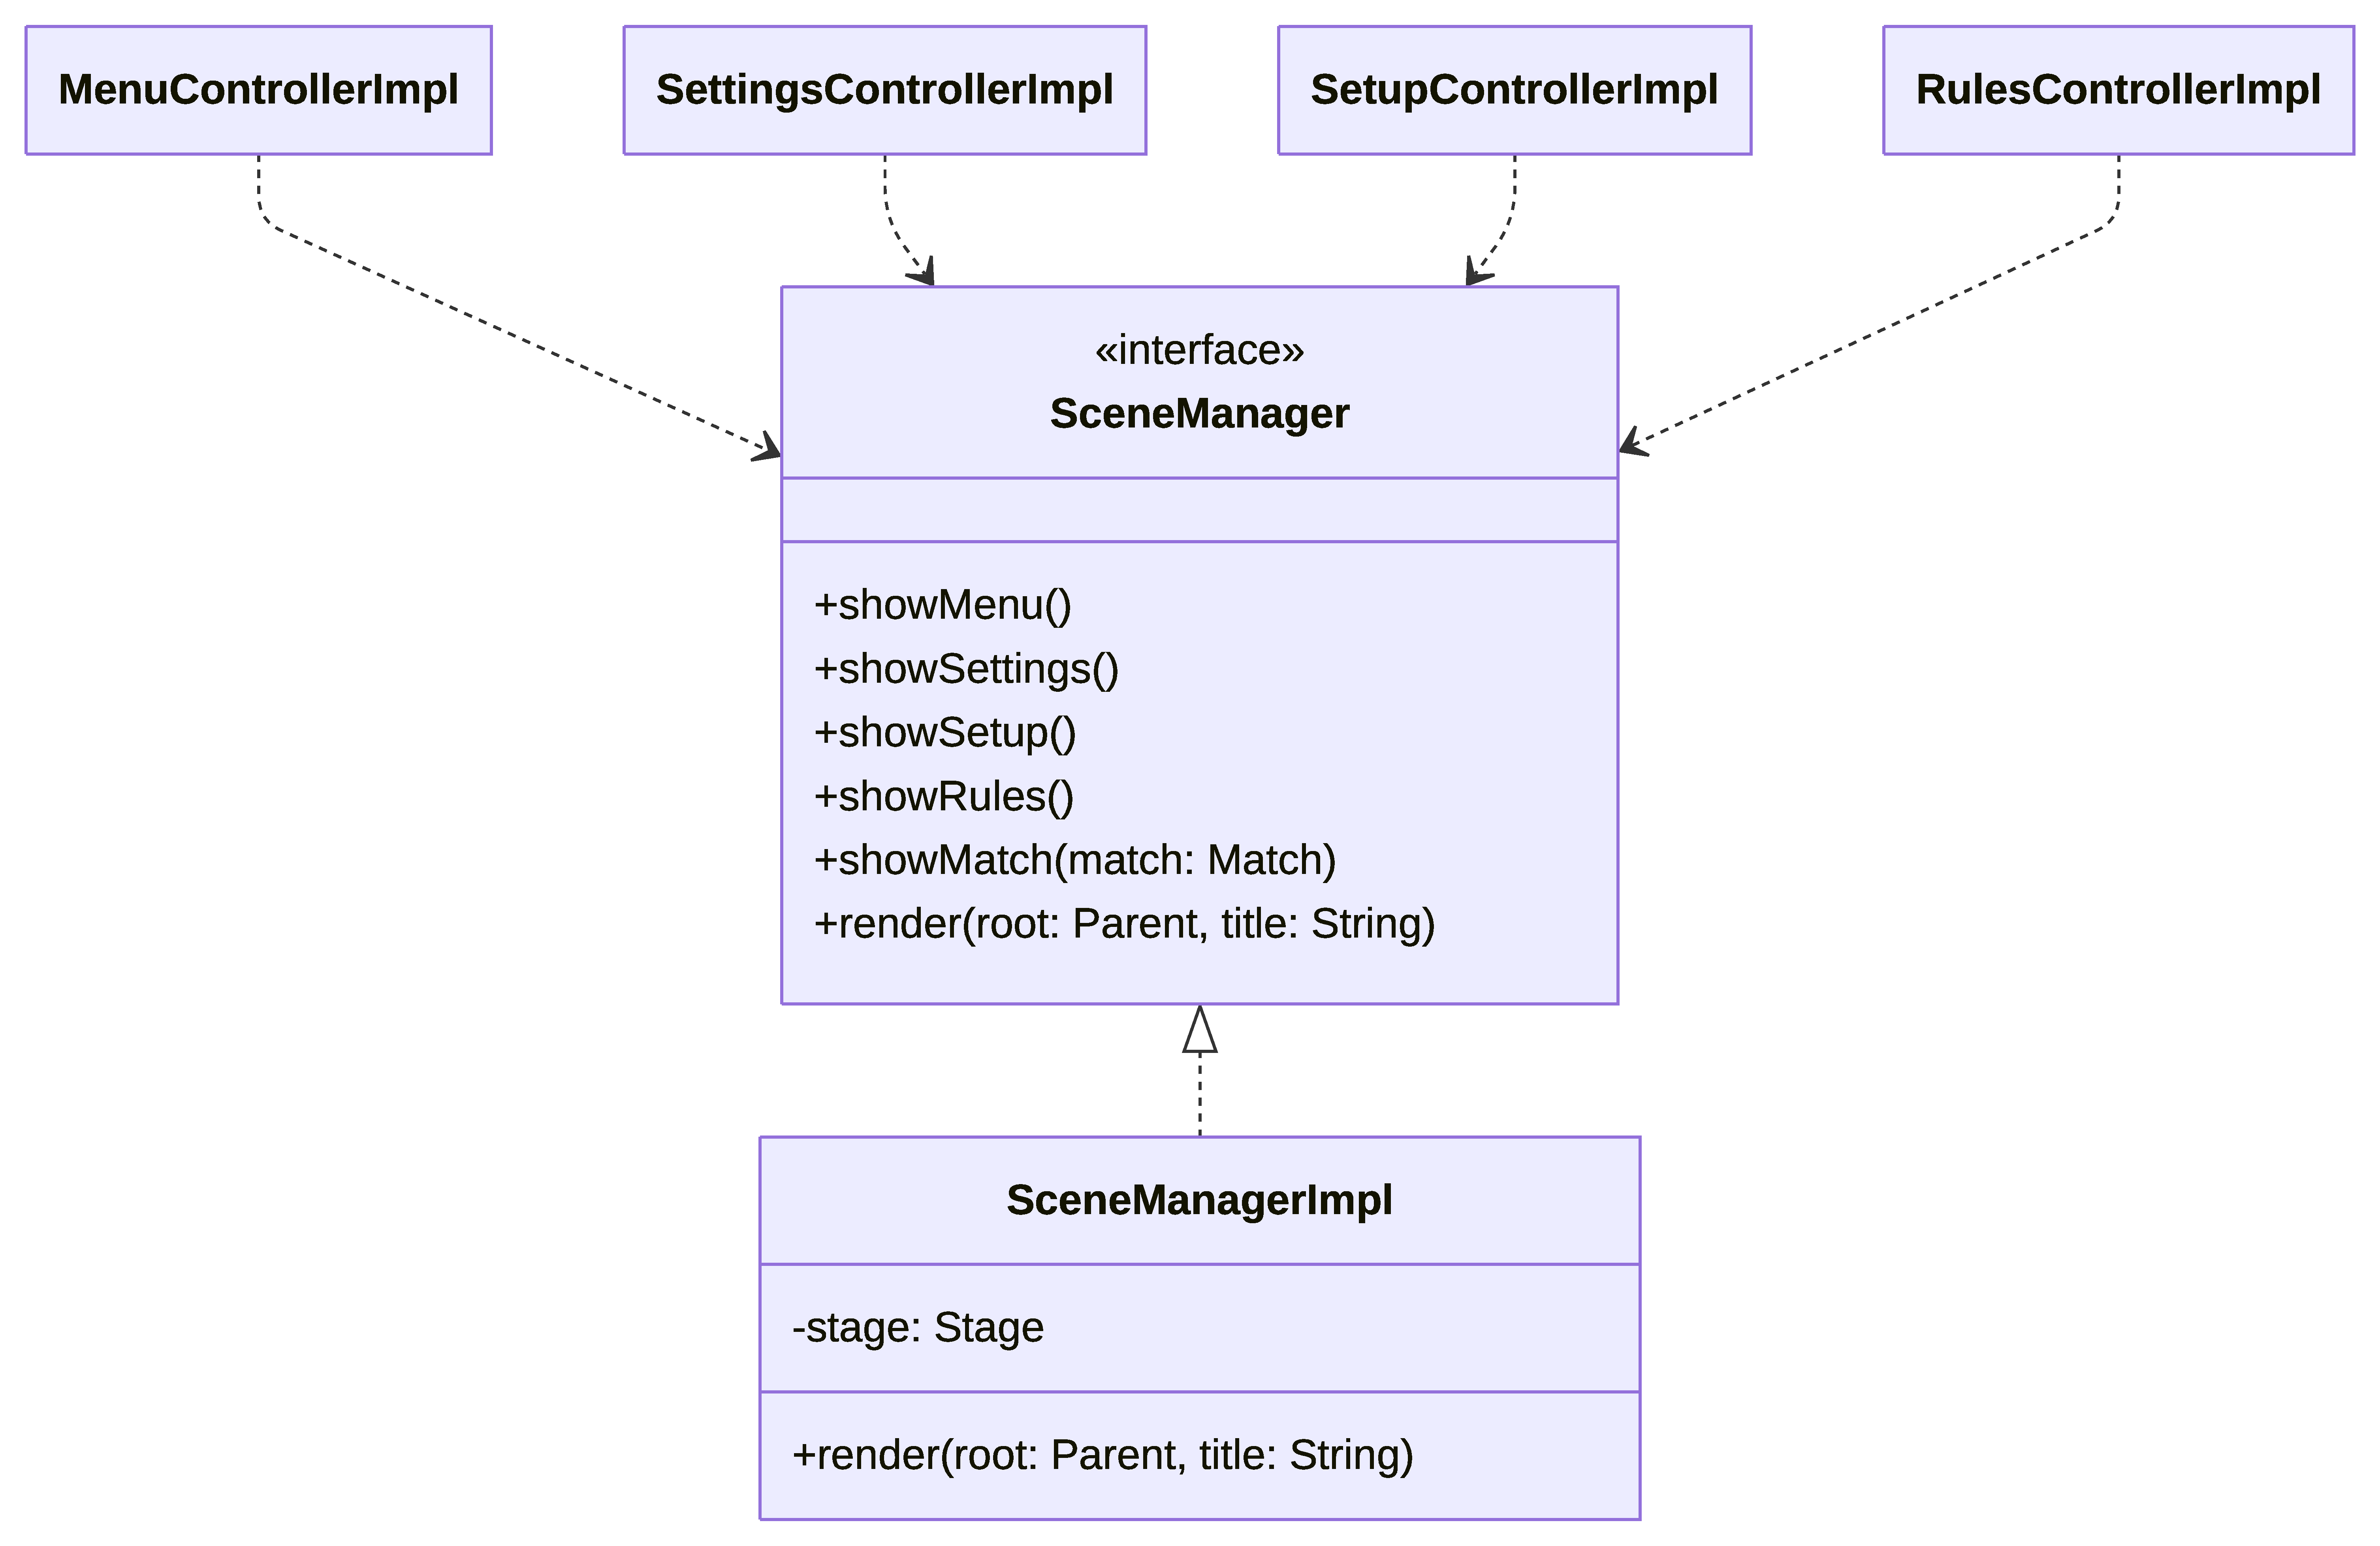
\includegraphics[width=\textwidth]{img/Figura2.2.pdf}
\caption{Il pattern Application Controller applicato alla navigazione. Ogni controller dipende solo dall'interfaccia \texttt{SceneManager}, eliminando le dipendenze circolari.}
\label{img:strategy}
\end{figure}

\paragraph{Problema} Nelle fasi iniziali di sviluppo della GUI, ogni vista era gestita dal proprio controller (es. \texttt{MenuController}, \texttt{SettingsController}). Per poter tornare alle schermate precedenti (ad esempio dalle impostazioni al menu), i controller dovevano istanziare altri controller passandosi reciprocamente riferimenti come argomenti del costruttore. Questo creava un forte accoppiamento e dipendenze circolari (ad esempio \texttt{SettingsController} dipendeva da \texttt{MenuController} e viceversa). La logica di navigazione e la gestione della finestra principale (\texttt{Stage}) risultavano frammentate e distribuite tra le varie classi.

\paragraph{Soluzione} È stata creata l'interfaccia \texttt{SceneManager} e la sua implementazione concreta \texttt{SceneManagerImpl}, che funge da Application Controller (una specializzazione del pattern Mediator): è l'unica classe a detenere il riferimento allo \texttt{Stage} di JavaFX. Tutti i controller dipendono esclusivamente dall'interfaccia \texttt{SceneManager}. Le View costruiscono il proprio albero grafico e invocano \texttt{sceneManager.render(root, title)}, che si limita a sostituire la root della scena (senza aprire nuove finestre). Questo ha eliminato totalmente l'accoppiamento: nessun controller conosce l'esistenza degli altri; ad esempio, quando l'utente preme "Impostazioni", il controller del menu chiama semplicemente \texttt{sceneManager.showSettings()}.


\subsubsection{Generazione e posizionamento delle caselle speciali (Strategy)}

\begin{figure}[H]
\centering{}
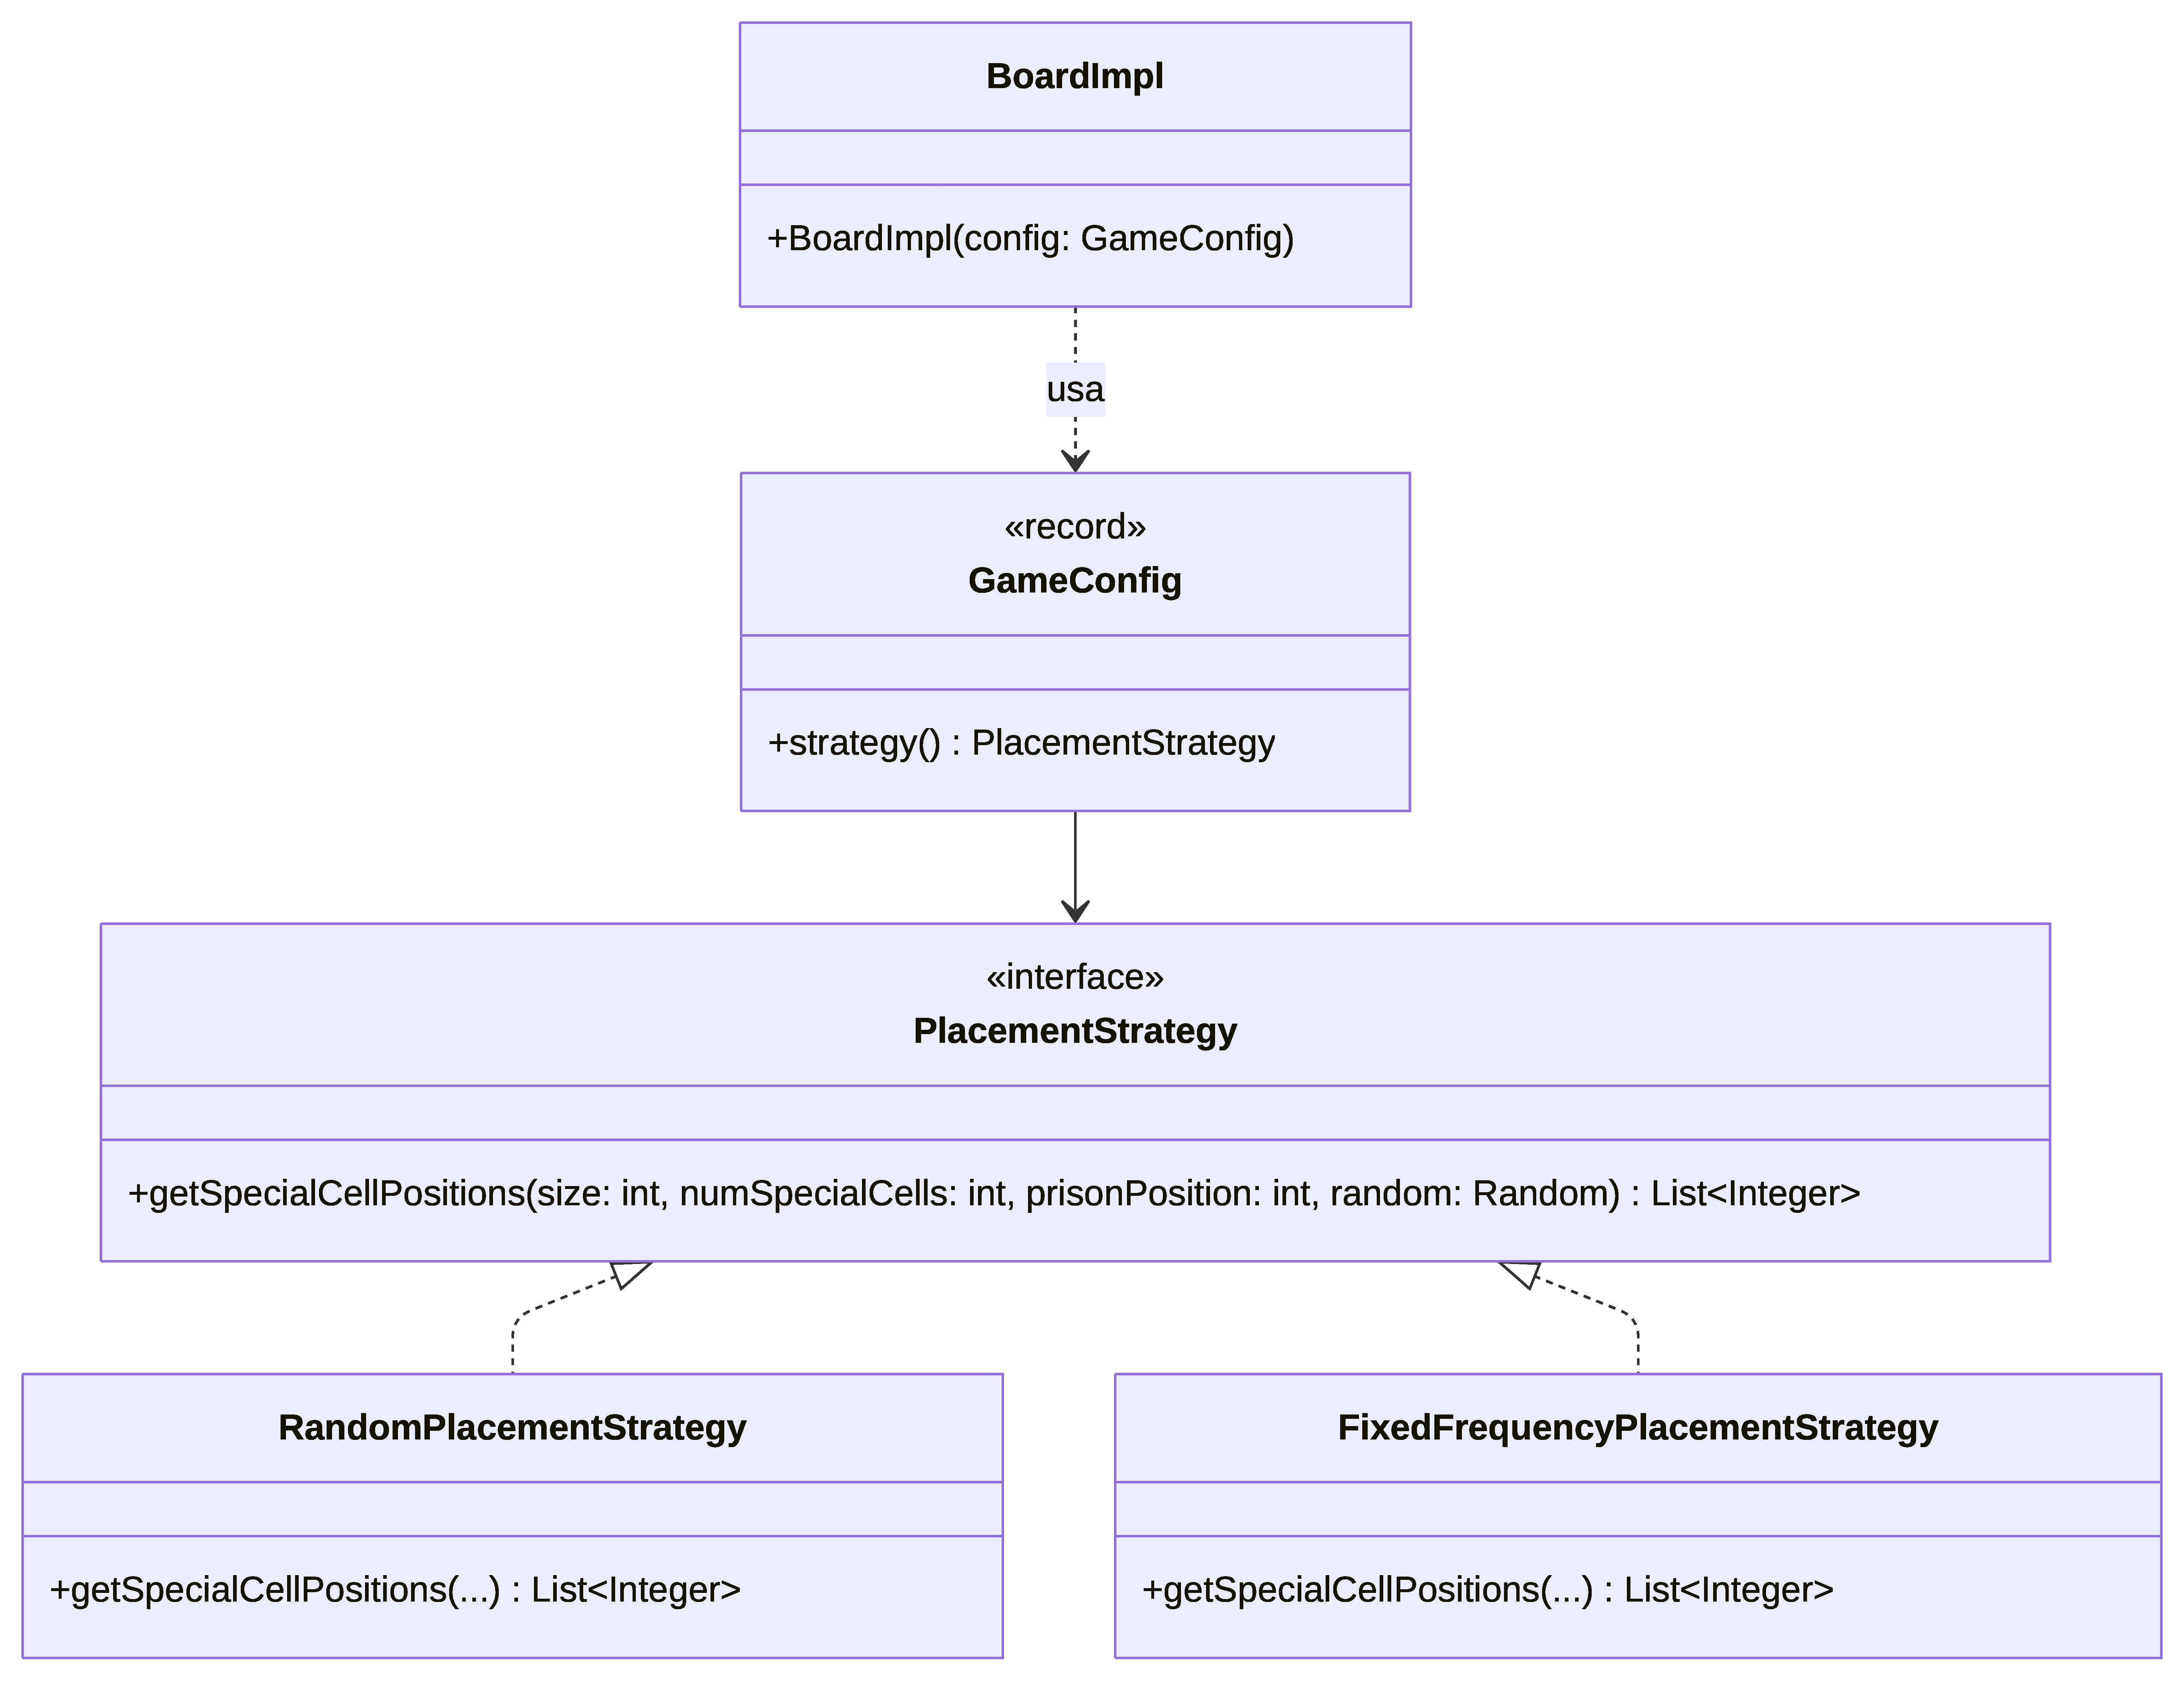
\includegraphics[width=\textwidth]{img/Figura2.3.pdf}
\caption{Il pattern Strategy per il posizionamento delle caselle speciali. \texttt{BoardImpl} delega la scelta delle posizioni all'interfaccia \texttt{PlacementStrategy}.}
\label{}
\end{figure}
\newpage
\paragraph{Problema} Il gioco richiede caselle speciali distribuite lungo il tabellone. L'utente può scegliere tra diverse modalità di distribuzione (casuale o a intervalli regolari), e si desidera poter aggiungere in futuro nuovi algoritmi di posizionamento senza modificare la classe \texttt{BoardImpl}, nel rispetto del principio Open/Closed.

\paragraph{Soluzione} È stato adottato il pattern \textbf{Strategy}. L'interfaccia \\\texttt{PlacementStrategy} definisce il contratto tramite il metodo \\\texttt{getSpecialCellPositions(...)}. Sono state implementate due strategie concrete: \texttt{RandomPlacementStrategy} (posizioni casuali) e \\\texttt{FixedFrequencyPlacementStrategy} (distribuzione a intervalli regolari). La strategia scelta viene iniettata nel record \texttt{GameConfig}, che a sua volta è passato a \texttt{BoardImpl} al momento della costruzione del tabellone. \texttt{BoardImpl} è il Context del pattern: invoca \\\texttt{config.strategy().getSpecialCellPositions(...)} senza conoscere quale strategia concreta sia in uso.

\subsubsection{Gestione centralizzata dell'audio (Singleton)}

\begin{figure}[H]
\centering{}
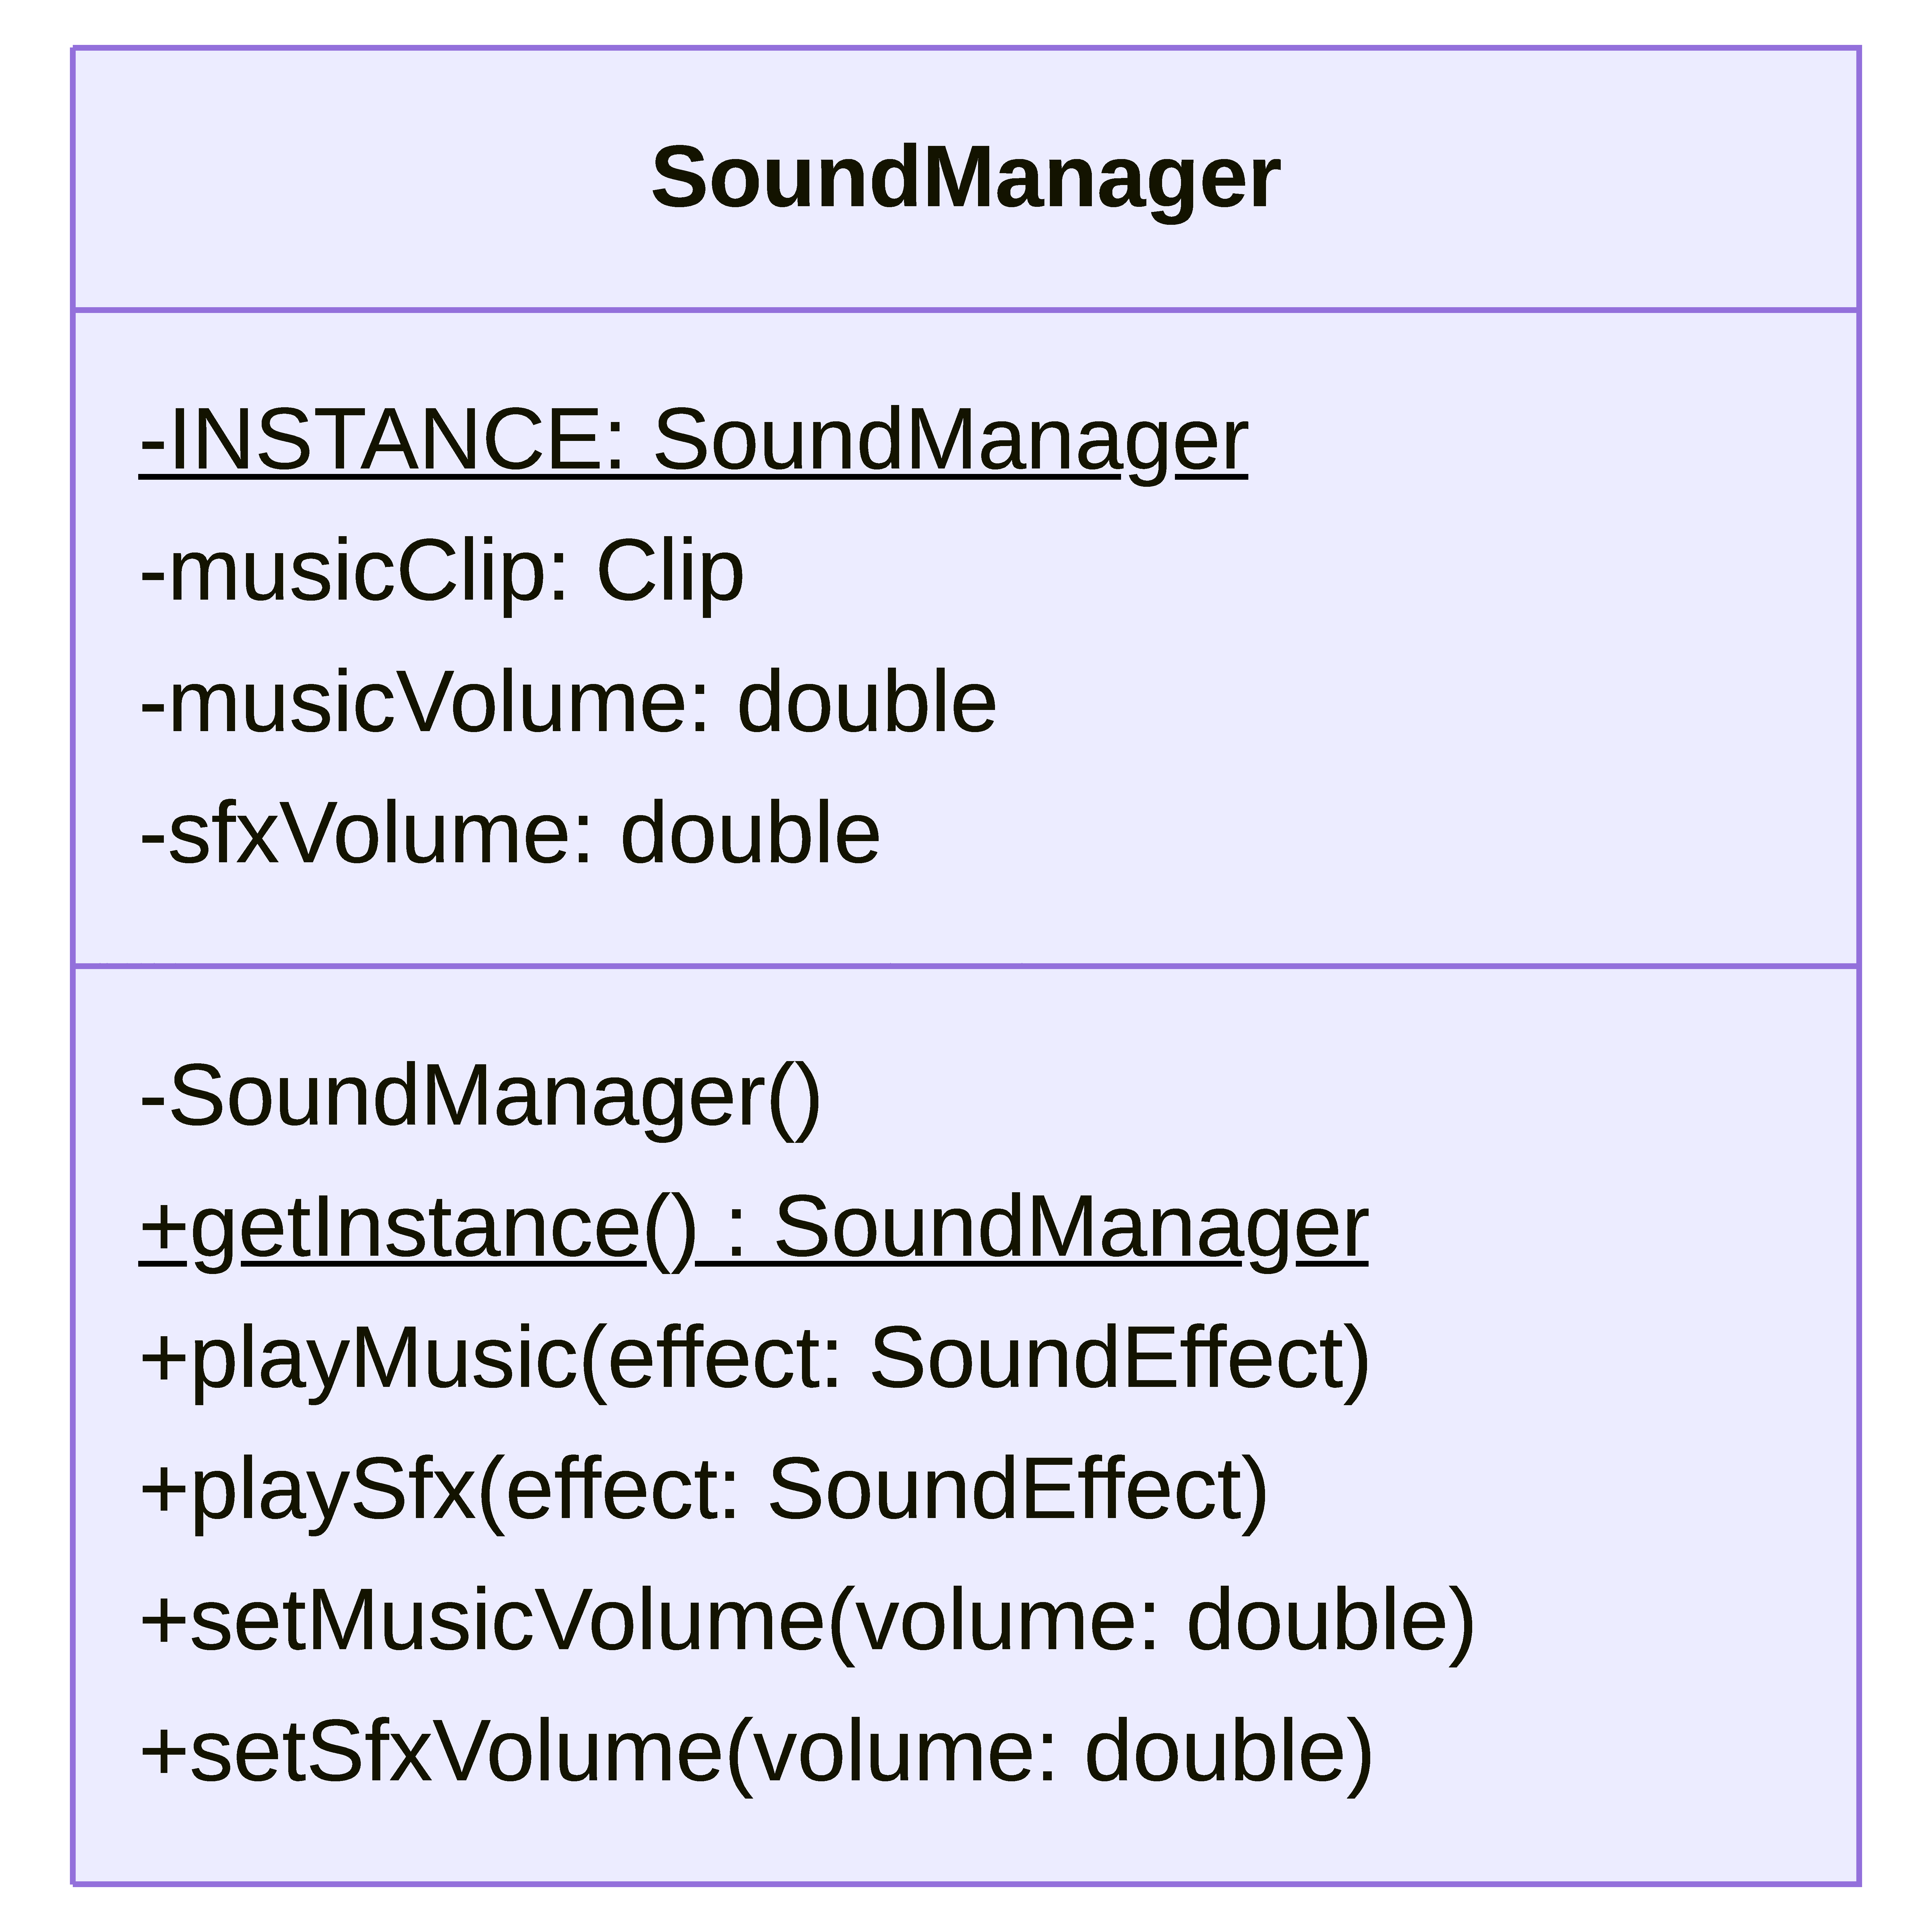
\includegraphics[width=.5\textwidth]{img/Figura2.4.pdf}
\caption{La classe \texttt{SoundManager} implementa il pattern Singleton con eager initialization.}
\label{img:observer}
\end{figure}
\newpage
\paragraph{Problema} Il sistema necessita di riprodurre effetti sonori (es. movimento pedine, vittoria) e musica di sottofondo da molteplici punti dell'applicazione (animazioni nella View, logica nel Controller). Istanziare una nuova classe per l'audio ad ogni riproduzione provocava desincronizzazioni e latenza. Passare un'istanza del manager audio come parametro a tutti i Controller e a tutte le View avrebbe inutilmente inquinato i costruttori.

\paragraph{Soluzione} È stato impiegato il pattern \textbf{Singleton} per la classe SoundManager. Un campo statico privato \texttt{INSTANCE} viene inizializzato al caricamento della classe; il costruttore è privato e il metodo statico \texttt{getInstance()} restituisce il riferimento all'unica istanza. Questo garantisce un solo punto di accesso globale al sistema audio e che le risorse vengano caricate ed eseguite nello stesso contesto, minimizzando la latenza e impedendo la frammentazione del volume tra istanze diverse.

\subsubsection{Effetti delle caselle intercambiabili (Strategy)}

\begin{figure}[H]
\centering{}
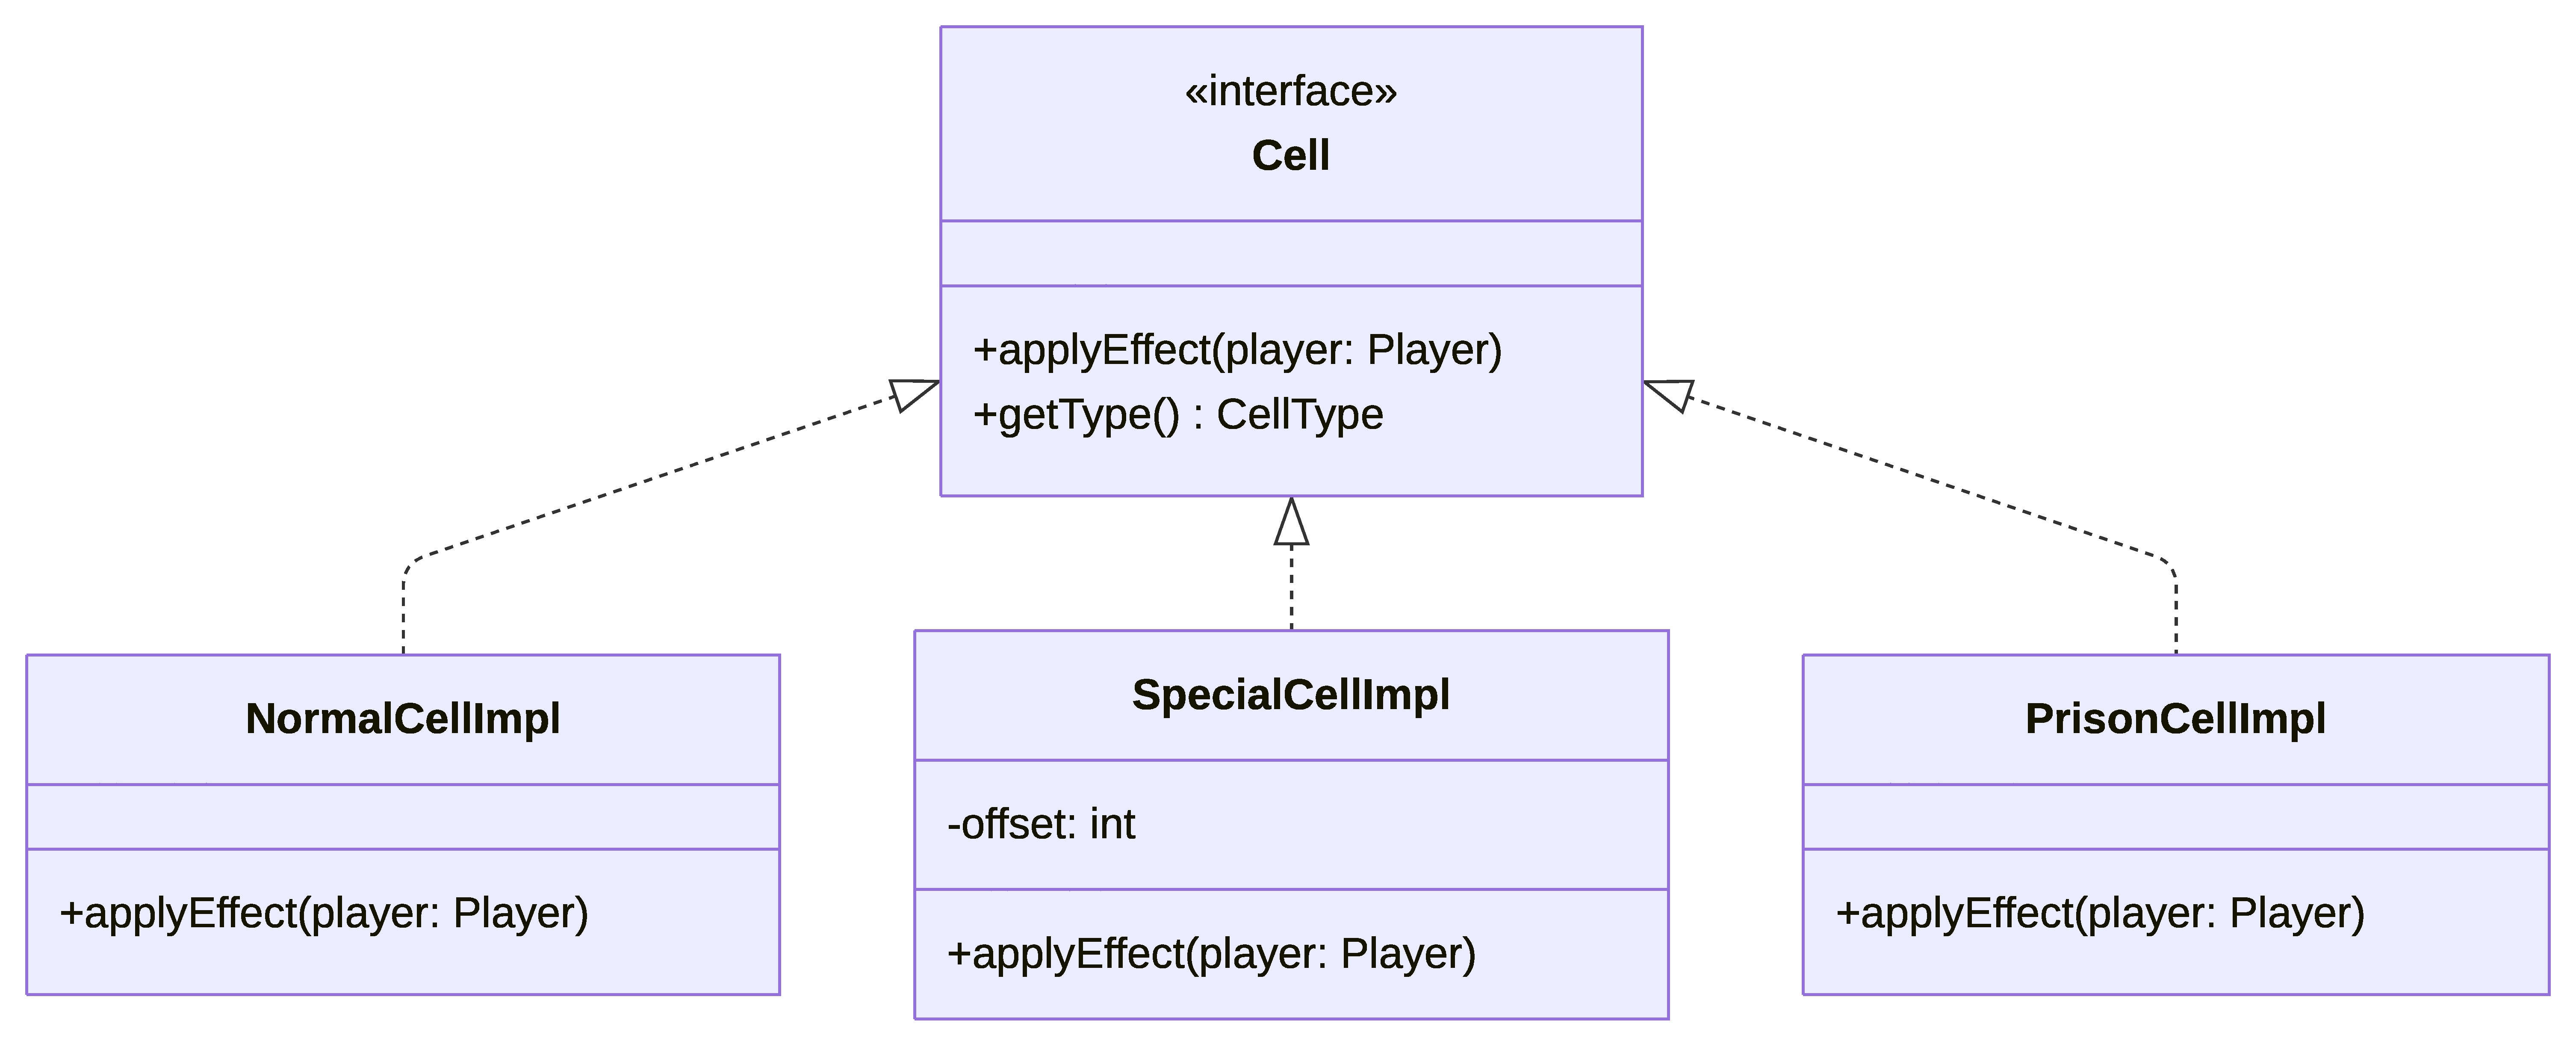
\includegraphics[width=\textwidth]{img/Figura2.5.pdf}
\caption{Il pattern Strategy applicato alle caselle. L'interfaccia \texttt{Cell} definisce il contratto \texttt{applyEffect(Player)} e ogni implementazione incapsula un diverso effetto di gioco.}
\label{img:observer}
\end{figure}

\paragraph{Problema}Il tabellone è composto da diverse tipologie di caselle (Normale, Speciale, Prigione), ciascuna con un effetto diverso sul giocatore che vi atterra. Gestire questi effetti tramite costrutti condizionali nel motore di partita (ad esempio uno \texttt{switch} sul tipo di casella in \texttt{MatchImpl}) avrebbe concentrato troppa logica nel controller e reso il sistema fragile: aggiungere una nuova tipologia di casella avrebbe richiesto di modificare il codice esistente, violando il principio Open/Closed.

\paragraph{Soluzione}È stato applicato il pattern Strategy all'interfaccia \texttt{Cell}, che dichiara il metodo \texttt{applyEffect(Player player)}. Ogni tipologia di casella è una strategia concreta che incapsula il proprio comportamento: \texttt{NormalCellImpl} non produce alcun effetto, \texttt{SpecialCellImpl} sposta il giocatore di un offset (bonus o malus), e \texttt{PrisonCellImpl} blocca il giocatore per un turno. Il motore di partita (\texttt{MatchImpl}) si limita a invocare \texttt{cell.applyEffect(player)} sulla casella corrente, senza dover conoscere il tipo concreto. Per aggiungere una nuova dinamica di gioco (ad esempio una casella che teletrasporta il giocatore) è sufficiente creare una nuova implementazione di \texttt{Cell}, senza toccare nessuna classe esistente

\subsection{Antonino Cardillo}
\subsubsection{Movimento della pedina, rimbalzo finale e gestione delle caselle speciali (`MatchImpl`)}


\begin{figure}[H]
\centering{}
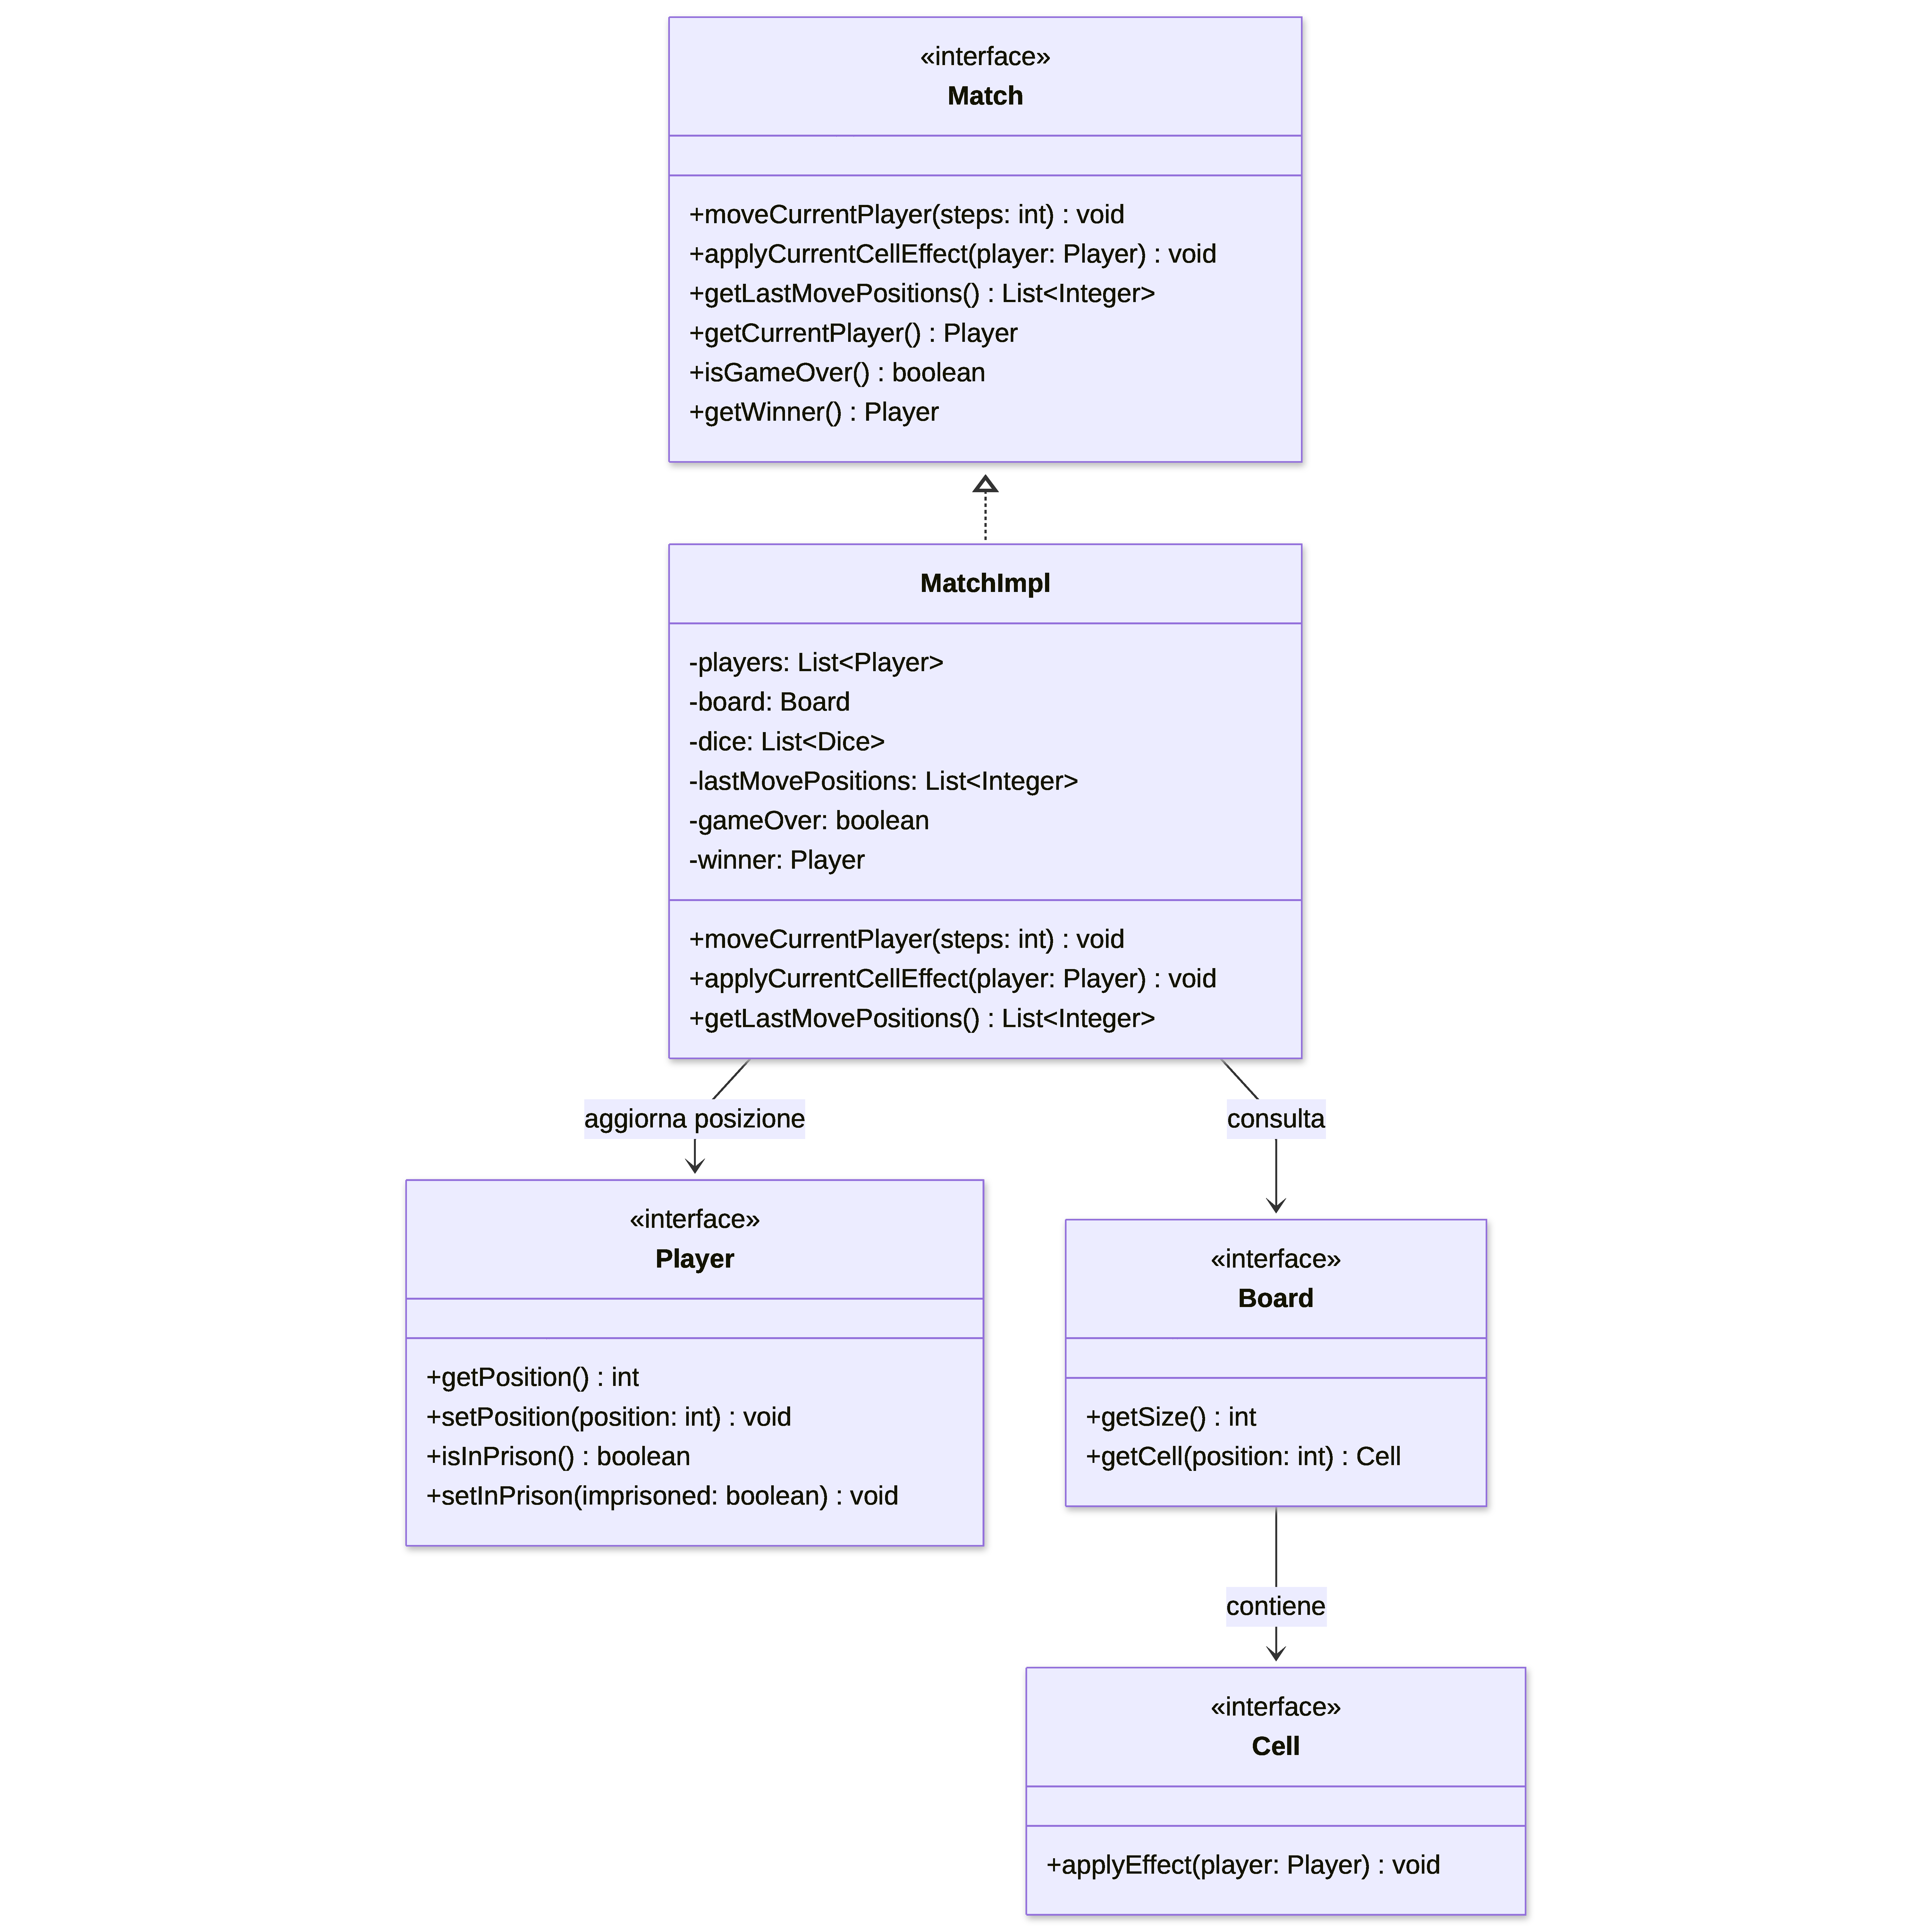
\includegraphics[width=\textwidth]{img/Figura2.6.pdf}
\caption{Schema della gestione del movimento e degli effetti in MatchImpl.}
\label{img:Movimento pedina}
\end{figure}

\paragraph{Problema:}Nel Gioco dell'Oca il movimento della pedina dopo il lancio del dado oltre ad avanzare sul percorso aggiungendo alla posizione attuale il risultato del dado, bisogna tener conto anche di alcuni aspetti di seguito elencati:
\begin{itemize}
	\item \textbf{Regola del rimbalzo:} per vincere la partita bisogna arrivare esattamente sulla casella (default 63 l'ultima). Se il punteggio del dado porta il giocatore oltre la casella 63, i passi in più devono essere fatti tornando indietro (ad esempio: se un giocatore è sulla casella 60 e fa 5 con il dado, arriva alla 63 e poi rimbalza indietro di 2 passi, fermandosi sulla 61).
    \item \textbf{Caselle speciali a catena:} se una pedina atterra su una casella speciale, subisce un effetto che la sposta in avanti (bonus) o indietro (malus). Questo nuovo spostamento potrebbe farla atterrare su un'altra casella speciale, innescando un secondo salto, oppure portarla sulla casella prigione. Inoltre c'e il rischio che, posizionando caselle speciali casuali, si può creare un ciclo infinito (ad esempio una casella che manda avanti di 2 e subito dopo una che manda indietro di 2), bloccando il gioco, questo anche nel caso si atterri su più caselle speciali in sequenza e se per il calcolo matematico si ritorna su quella di partenza si crea un loop.
    \item \textbf{Tracciamento per la grafica:} per rendere la parte grafica inerente alla parte logica, la parte grafica deve conoscere non solo la posizione finale, ma tutti i singoli salti intermedi effettuati dalla pedina (il tocco del 63, il rimbalzo, i salti delle caselle speciali), così da poterli mostrare uno dopo l'altro al giocatore con le giuste animazioni e i giusti suoni.
\end{itemize}
\paragraph{Soluzione:}La logica è tutta protetta all'interno del modello della classe \texttt{MatchImpl}, utilizzando il principio dell'incapsulamento, nei metodi \texttt{moveCurrentPlayer(int steps)} e \texttt{applyCurrentCellEffect(Player player)} in quest'ultima viene sfruttato il polimorfismo delle diverse tipologie di casella senza ricorrere a controlli con il costrutto if-else sul tipo di cella. Non ci sono rischi di blocchi o crash per cicli infiniti. La grafica riceve la sequenza precisa dei salti da animare. Nello specifico viene dettagliato di seguito:
  \begin{itemize}
    \item Quando si muove il giocatore, se la nuova posizione supera la fine del percorso (63), calcolo l'eccesso e faccio arretrare la pedina (63 - eccesso), aggiungendo sia la casella finale che quella di arrivo a una lista dei movimenti \texttt{lastMovePositions}.
    \item Per gli effetti delle caselle speciali, ho usato un ciclo \texttt{while} che continua finchè la pedina si sposta. Per evitare che un giro vizioso di caselle speciali blocchi il programma in un loop infinito, salvo ogni casella visitata in un hashMap \texttt{Set<Integer> visitedPositions}, se la pedina ricapita su una casella già toccata nello stesso turno, il ciclo si interrompe subito.
    \item Come già anticipato, tutte le posizioni toccate nel turno vengono salvate nella lista \texttt{lastMovePositions}. All'esterno la espongo con il metodo \texttt{getLastMovePositions()}, restituendo una lista non modificabile \texttt{Collections.unmodifiableList} in modo che nessun'altra classe possa alterarla per errore.
  \end{itemize}

\subsubsection{Gestione dei tempi, animazioni e messaggi nel Controller (`MatchControllerImpl`)}
 \begin{figure}[H]
 \centering{}
 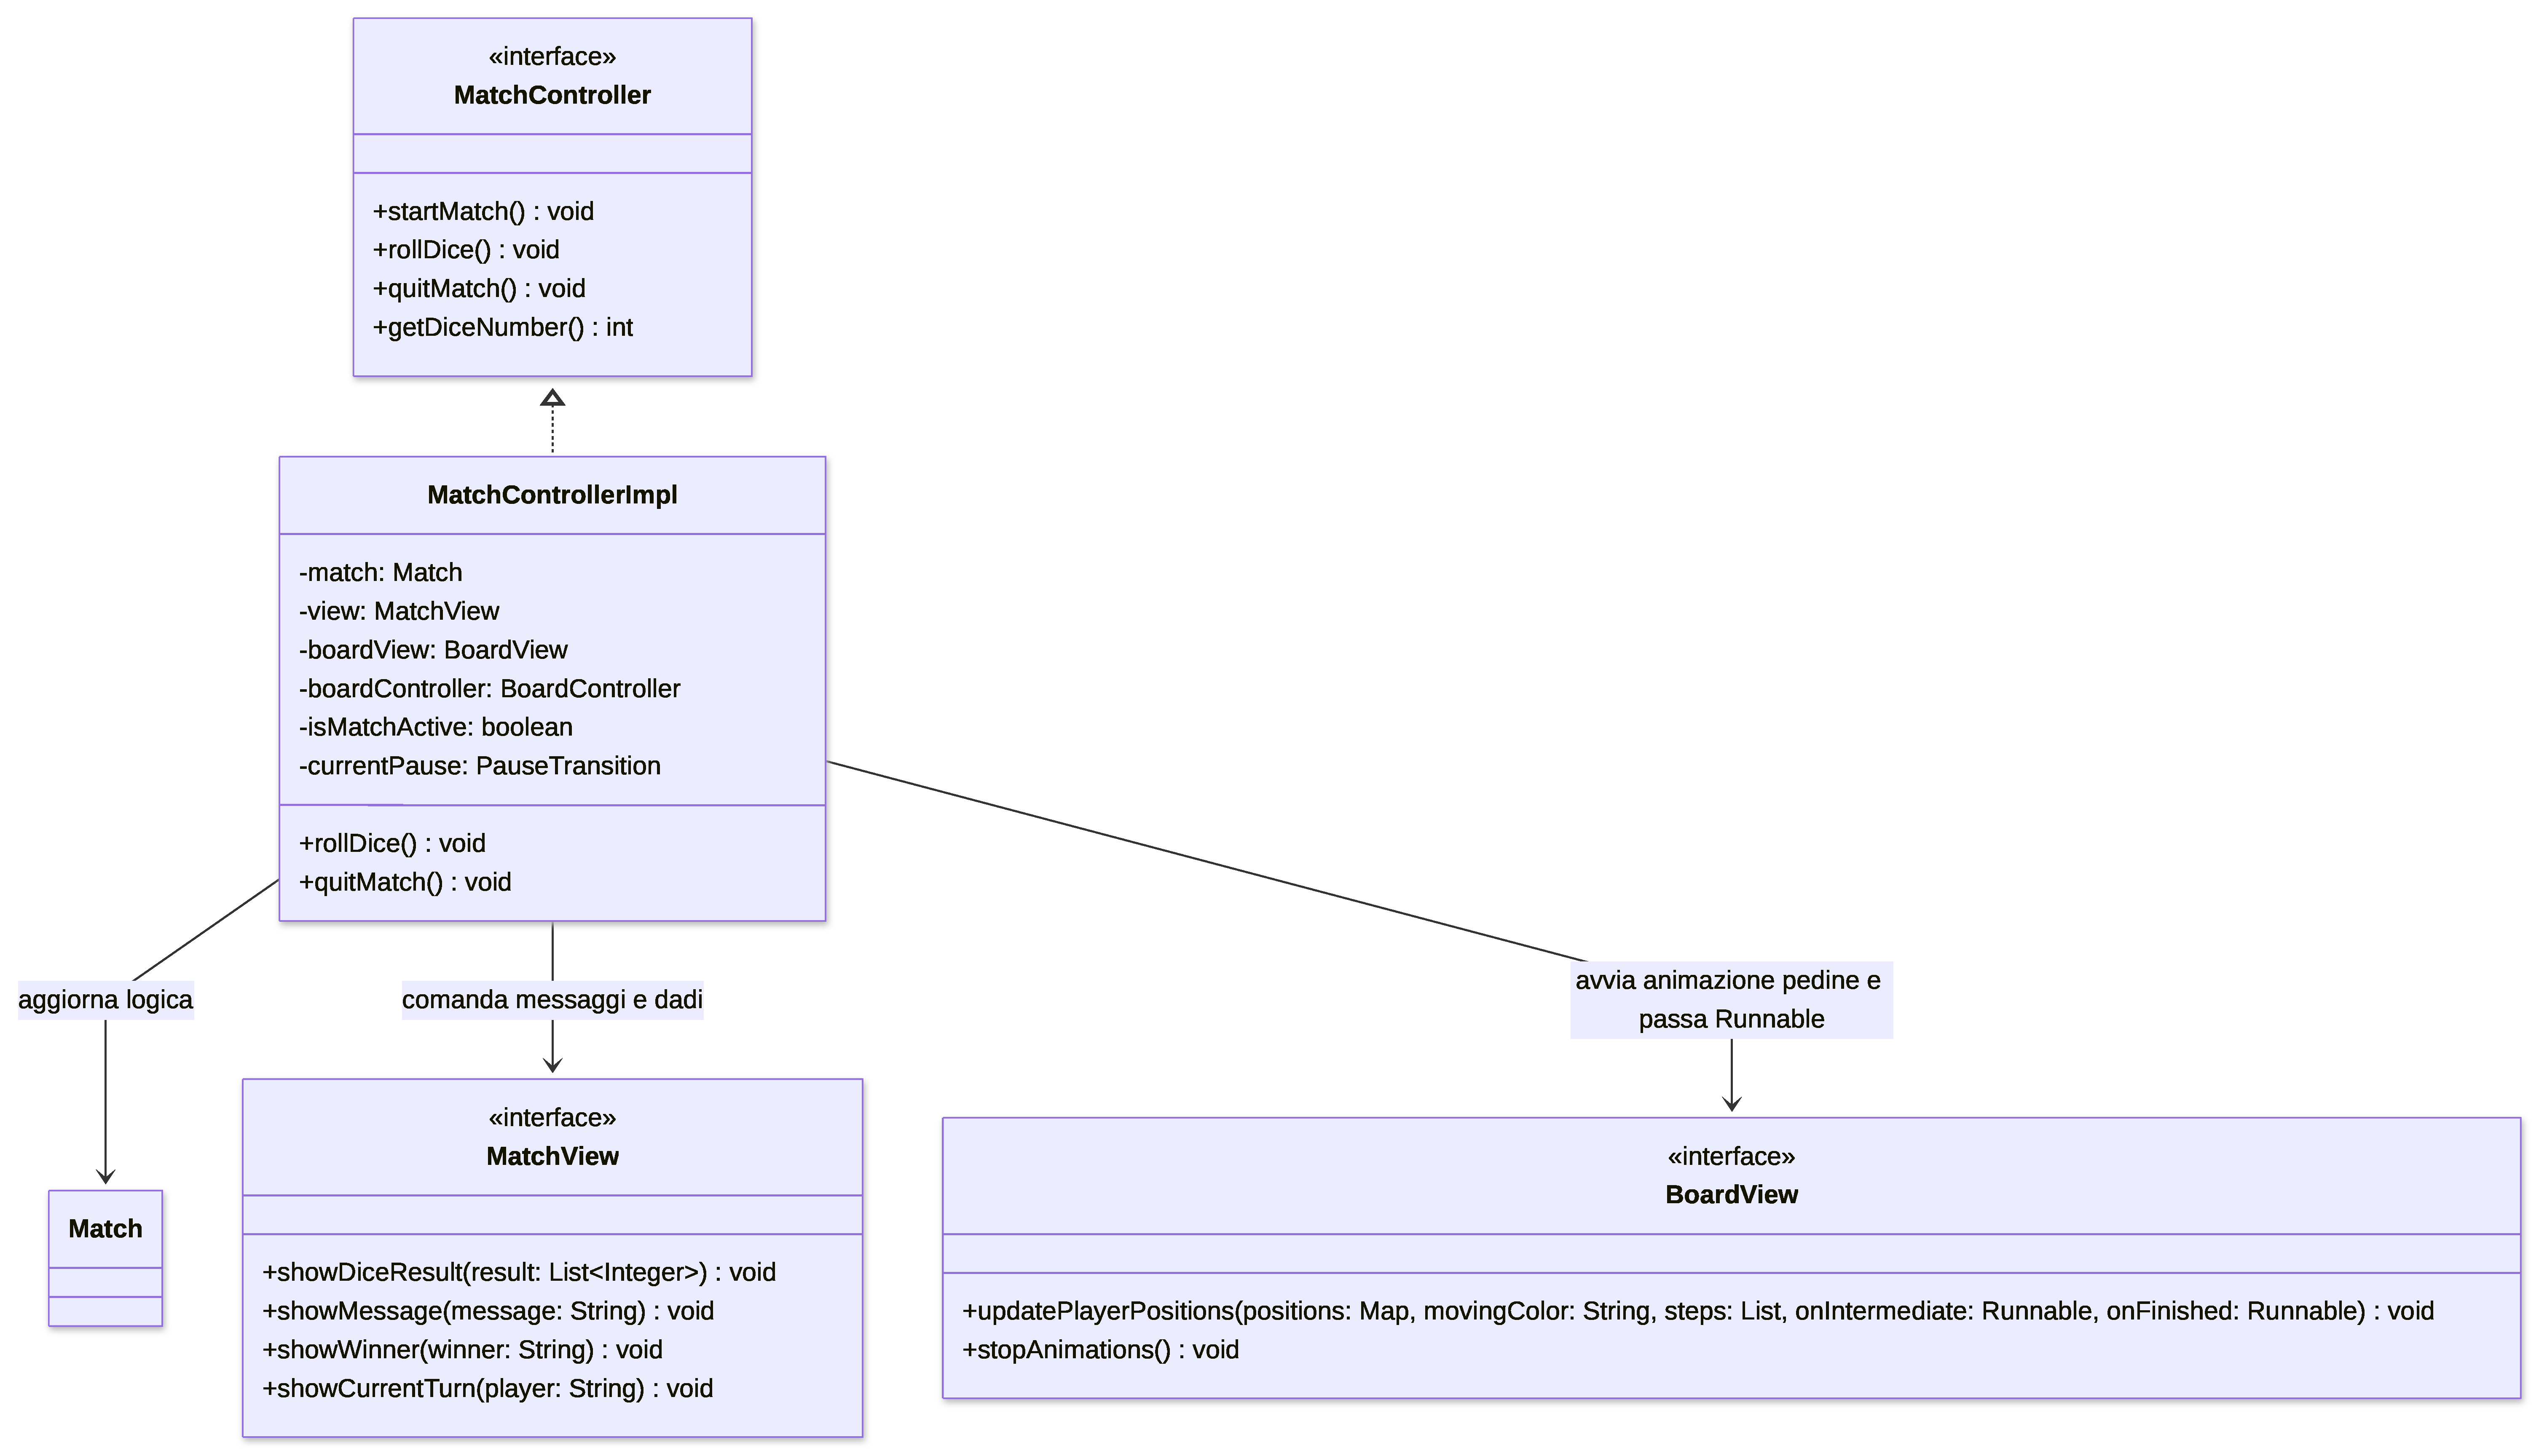
\includegraphics[width=\textwidth]{img/Figura2.7.pdf}
 \caption{Schema della gestione del movimento e degli effetti in MatchImpl.}
 \label{img:Gestione Effetti}
 \end{figure} 
 \paragraph{Problema:}Quando il giocatore clicca sul pulsante per lanciare il dado, succedono varie cose in sequenza:
 \begin{enumerate}
     \item Si deve vedere l'animazione dei dadi che rotolano e sentire il suono del lancio.
     \item Bisogna aspettare che i dadi abbiano finito di girare prima di far partire la pedina.
     \item La pedina deve avanzare sul percorso; se tocca una casella speciale o rimbalza, deve riprodurre il suono adatto (suono a molla per il rimbalzo, suono speciale per il bonus/malus).
     \item Quando il movimento è del tutto concluso, bisogna scrivere nella finestra di log cosa è successo (es. *"Rimbalzo!"*, *"Ops, sei finito in prigione!"*), verificare se il giocatore ha vinto o passare il turno a quello successivo.
 \end{enumerate}
  In JavaFX tutte le modifiche grafiche avvengono su un unico thread (il thread dell'interfaccia grafica). Se avessi usato un comando bloccante come \texttt{Thread.sleep()}, l'intera applicazione si sarebbe congelata: la finestra sarebbe andata in blocco con il classico \texttt{("Non risponde")} e le animazioni non si sarebbero viste. Inoltre, per il pattern MVC la vista del tabellone \texttt{(BoardView)} non doveva conscere i testi dei messaggi, dei turni o delle regole di vittoria.
  \paragraph{Soluzione:}Ho utilzzato le classi di animazione di JavaFx e usato le \texttt{CallBack} passandole come parametro tramite \texttt{Runnable} insieme alla lista dei salti alla view \texttt{BoardView} con il metodo \texttt{updatePlayerPositions}.
  Nel momento del lancio, la vista \texttt{MatchViewImpl} fa partire un'animazione \textbf{Timeline} per cambiare velocemente le facce dei dadi.
  Nel controller uso \texttt{PauseTransition} della durata di un secondo, che aspetta la fine del lancio dei dadi senza bloccare la finestra. Finita la pausa, il controller chiede al modello di muovere la pedina e chiama il metodo \texttt{boardView.updatePlayerPositions(...)}, passandogli due azioni da eseguire:
    Azione intermedia \texttt{(onIntermediate)}, la vista del tabellone la richiama ogni volta che la pedina raggiunge un punto intermedio, permettendo al controller di riprodurre il suono corretto (molla per il rimbalzo o suono speciale per le celle bonus/malus);
    Azione finale \texttt{(onFinal)}, la vista del tabellone la richiama solo quando la pedina è ferma sulla casella finale, permettendo al controller di stampare i messaggi di testo nel log, suonare la vittoria se la partita è finita, oppure passare il turno con \texttt{match.nextTurn()}.

\chapter{Sviluppo}
\section{Testing automatizzato}

Il testing automatizzato si è concentrato sulle componenti del modello di dominio, utilizzando il framework JUnit 5. In particolare sono stati verificati:

\begin{itemize}
 \item \textbf{BoardImplTest:} correttezza della generazione del tabellone (dimensione, presenza della casella prigione nella posizione attesa, distribuzione delle caselle speciali in base alla strategia).
 \item \textbf{PlayerImplTest:} inizializzazione dello stato del giocatore, gestione della posizione e dello stato di prigione.
 \item \textbf{DiceImplTest:} verifica che i valori generati dal dado rientrino nell'intervallo atteso.
 \item \textbf{SpecialCellImplTest:} applicazione corretta dell'offset (bonus e malus), inclusi i controlli sui limiti del tabellone.
 \item \textbf{PrisonCellImplTest:} verifica che l'effetto della cella prigione metta correttamente il giocatore in stato \texttt{inPrison}.
 \item \textbf{NormalCellImplTest:} verifica che la casella normale non alteri la posizione del giocatore.
 \item \textbf{MatchImplTest:} Contiene più test, viene verificato \texttt{l'inizializzazione del Match},  il \texttt{player che inizia}, il suo \texttt{nickName}, lo stato di \texttt{GameOver(false)} e di \texttt{Vittoria(null)}, il \texttt{numero di giocatori}, la \texttt{posizione iniziale del giocatore}, il \texttt{turno}, l'applicazione della \texttt{cella speciale}. 
\end{itemize}



\section{Note di sviluppo}
\subsection{Nicolae Balaban}
\subsubsection{Uso di lambda expressions}
Impiegate in maniera pervasiva per la gestione reattiva degli eventi grafici, rendendo il codice significativamente più conciso rispetto all'utilizzo di classi anonime.\\
\href{https://github.com/Nick-2002b/PSS25-Gioco-Oca/blob/e81943445d44f9befaaf74b02e1793cb20d0ce74/src/main/java/it/unibo/giocooca/view/impl/SettingsViewImpl.java#L97}{Permalink}

\subsubsection{Uso di switch expressions (arrow syntax)}
Utilizzate per migliorare la leggibilità e ridurre le possibilità di errori da fall-through, sfruttando la sintassi -$>$ introdotta in Java 14+.\\
\href{https://github.com/Nick-2002b/PSS25-Gioco-Oca/blob/e81943445d44f9befaaf74b02e1793cb20d0ce74/src/main/java/it/unibo/giocooca/view/impl/BoardViewImpl.java#L117-L122}{Permalink}

\subsubsection{Uso di Java Records}
Il costrutto \texttt{record} è stato sfruttato per definire piccole classi portatrici di dati immutabili, eliminando il boilerplate (costruttori, getter, \texttt{equals}, \texttt{hashCode}). Usato sia nel model (\texttt{GameConfig}) sia nella view (\texttt{LogicalCoords}, \texttt{GridCoords} in \texttt{BoardViewImpl}).\\
\href{https://github.com/Nick-2002b/PSS25-Gioco-Oca/blob/e81943445d44f9befaaf74b02e1793cb20d0ce74/src/main/java/it/unibo/giocooca/view/impl/BoardViewImpl.java#L430-L434)}{Permalink}

\subsubsection{Pattern Matching for \texttt{instanceof}}
Utilizzato per il cast sicuro e conciso, evitando la verbosità del check e cast su due righe separate.\\
\href{https://github.com/Nick-2002b/PSS25-Gioco-Oca/blob/e81943445d44f9befaaf74b02e1793cb20d0ce74/src/main/java/it/unibo/giocooca/navigation/impl/SceneManagerImpl.java#L84}{Permalink}

\subsubsection{Uso della libreria \texttt{javax.sound.sampled}}
Parte della JDK ma non trattata a lezione. Utilizzata in SoundManager per la riproduzione audio (\texttt{Clip}, \texttt{AudioSystem}, \texttt{FloatControl}) con gestione del volume in decibel.\\
\href{https://github.com/Nick-2002b/PSS25-Gioco-Oca/blob/e81943445d44f9befaaf74b02e1793cb20d0ce74/src/main/java/it/unibo/giocooca/audio/SoundManager.java#L136-L142}{Permalink}
\newpage
\subsubsection{Uso della libreria di terze parti JavaFX}
Impiegata come framework grafico per tutte le view. In particolare, le classi di animazione (\texttt{TranslateTransition}, \texttt{SequentialTransition}, \texttt{PauseTransition}) sono state utilizzate per il movimento delle pedine sul tabellone.\\
\href{https://github.com/Nick-2002b/PSS25-Gioco-Oca/blob/e81943445d44f9befaaf74b02e1793cb20d0ce74/src/main/java/it/unibo/giocooca/view/impl/BoardViewImpl.java#L399-L403}{Permalink}

\subsection{Antonino Cardillo}
\subsubsection{Uso di lambda expressions}
Utilizzate in più occasione per la gestione degli eventi sia per le CallBack che per l'azione dei Button. \\

\noindent\textbf{CallBack MatchControllerImpl:}\\
 - setOnFinished
 \href{https://github.com/Nick-2002b/PSS25-Gioco-Oca/blob/e81943445d44f9befaaf74b02e1793cb20d0ce74/src/main/java/it/unibo/giocooca/controller/impl/MatchControllerImpl.java#L98}{Permalink} \\
 - onIntermediate
 \href{https://github.com/Nick-2002b/PSS25-Gioco-Oca/blob/e81943445d44f9befaaf74b02e1793cb20d0ce74/src/main/java/it/unibo/giocooca/controller/impl/MatchControllerImpl.java#L116}{Permalink} \\
 - onFinal
 \href{https://github.com/Nick-2002b/PSS25-Gioco-Oca/blob/e81943445d44f9befaaf74b02e1793cb20d0ce74/src/main/java/it/unibo/giocooca/controller/impl/MatchControllerImpl.java#L128}{Permalink} \\
\textbf{Button MatchViewImpl:}\\
- btnRollDice
\href{https://github.com/Nick-2002b/PSS25-Gioco-Oca/blob/e81943445d44f9befaaf74b02e1793cb20d0ce74/src/main/java/it/unibo/giocooca/view/impl/MatchViewImpl.java#L158}{Permalink}\\
- btnQuit
\href{https://github.com/Nick-2002b/PSS25-Gioco-Oca/blob/e81943445d44f9befaaf74b02e1793cb20d0ce74/src/main/java/it/unibo/giocooca/view/impl/MatchViewImpl.java#L163}{Permalink}\\

\subsubsection{Uso di librerie di terze parti JavaFx}
In MatchViewImpl per l' animazione dei dadi ho utilizzato \textett{Timeline} e \texttt{Keyframe} per alternare le facce del dado.
\href{https://github.com/Nick-2002b/PSS25-Gioco-Oca/blob/e81943445d44f9befaaf74b02e1793cb20d0ce74/src/main/java/it/unibo/giocooca/view/impl/MatchViewImpl.java#L224-L235}{Permalink}\\
In MatchControllerImpl ho utilizzato PauseTransition per avere una pausa tra l'animazione del dado e lo spostamento della pedina.
\href{https://github.com/Nick-2002b/PSS25-Gioco-Oca/blob/e81943445d44f9befaaf74b02e1793cb20d0ce74/src/main/java/it/unibo/giocooca/controller/impl/MatchControllerImpl.java#L96}{Permalink}\\

\chapter{Commenti finali}

\subsection{Nicolae Balaban}
\paragraph{Ruolo nel gruppo.}Ho rivestito il ruolo di responsabile della parte grafica e della struttura di navigazione dell'applicativo. Nello specifico, mi sono occupato dell'architettura di navigazione tra schermate (\texttt{SceneManager}), della realizzazione grafica del tabellone (\texttt{BoardViewImpl}), delle view per impostazioni e regole (\texttt{SettingsViewImpl}, \texttt{RulesViewImpl}), dell'implementazione delle classi del modello (\texttt{PlayerImpl}, \texttt{BoardImpl}, \texttt{DiceImpl}, le specializzazioni di \texttt{Cell}), del pattern Strategy per il posizionamento delle caselle speciali, e del sistema audio centralizzato (\texttt{SoundManager}).

\subsubsection{Punti di forza}
\begin{itemize}
    \item Il tabellone è completamente espandibile: l'interfaccia \texttt{Cell} e il metodo \texttt{applyEffect(Player)} permettono di aggiungere nuove tipologie di caselle senza alterare il motore di partita.
    \item Il pattern Strategy consente di aggiungere nuovi algoritmi di distribuzione delle caselle speciali senza toccare \texttt{BoardImpl}.
    \item L'architettura \texttt{SceneManager} ha eliminato completamente le dipendenze circolari tra controller, rendendo ogni controller indipendente dagli altri.
\end{itemize}

\subsubsection{Punti di debolezza}
\begin{itemize}
    \item Scrivere tutta la GUI in codice procedurale Java rende alcune classi View inevitabilmente prolisse rispetto a un approccio dichiarativo con markup.
    \item Migliorare la gestione della riproduzione degli effetti audio sfx perche' attualmente non la ritengo soddisfacente personalmente.
\end{itemize}

\paragraph{Lavori Futuri.}Si potrebbe estrapolare tutta la parte grafica usando fogli di stile CSS e layout FXML per una miglior separazione tra logica e presentazione. Si potrebbero inoltre aggiungere ulteriori dinamiche di gioco (nuove tipologie di caselle, modalità multigiocatore online) sfruttando l'estensibilità già predisposta dal modello.

\subsection{Antonino Cardillo}
\paragraph{Ruolo nel gruppo.} All'interno del progetto mi sono occupato principalmente della logica centrale della partita \textbf{(Match e MatchImpl)}, del coordinamento degli eventi di gioco tramite il controller \textbf{(MatchControllerImpl)}, dell'interfaccia principale della partita con l'animazione dei dadi \textbf{(MatchViewImpl)}, della schermata di registrazione iniziale dei giocatori \textbf{(SetupViewImpl e SetupControllerImpl)} e della stesura dei relativi test unitari con JUnit 5. 
La collaborazione con il mio collega Nicolae è stata costante e proficua: ci siamo suddivisi i compiti fin dall'inizio in modo chiaro (a lui la generazione del tabellone, la grafica della pista e l'audio; a me il motore della partita e il coordinamento del flusso di gioco). Abbiamo gestito l'integrazione del codice tramite Git e GitHub, discutendo insieme le interfacce per far dialogare le nostre componenti senza creare sovrapposizioni utilizzando classi mock.
\subsubsection{Punti di forza}
Ritengo che i principali punti di forza del mio lavoro siano, la logica di avanzamento in MatchImpl è robusta, protetta da loop infiniti grazie al controllo sulle caselle speciali già visitate, la registrazione dei giocatori impedisce errori banali, garantendo che ogni partecipante abbia un nome valido e un colore di pedina univoco, con poco sforzo aggiungere la possibilità di avere un dado a più di sei facce e un numero superiore di due.
\subsubsection{Punti di debolezza}
il metodo \texttt{rollDice} in \texttt{MatchControllerImpl} svolge molte mansioni (coordina pause, suoni, messaggi e avanzamento turno). Sebbene funzioni bene, in futuro potrebbe essere suddiviso in sotto-metodi più piccoli per renderlo ancora più pulito e modulare.
\paragraph{Lavori Futuri.}
Penso che si potrebbe ampliare le difficoltà con tipi di caselle speciali diverse, salvare lo stato del gioco per poterlo riprendere in seguito, banalmente su un file json, utilizzare il pattern Observer per la view. 

\section{Difficoltà incontrate e commenti per i docenti}
\subsection{Nicolae Balaban}
La difficoltà principale ha riguardato la realizzazione grafica del tabellone a "serpentone". Il percorso del gioco dell'oca prevede righe dritte separate da caselle d'angolo, con direzione alternata. Si è resa necessaria una netta separazione tra coordinate logiche (dove sta una casella nel percorso) e coordinate della griglia (come \texttt{GridPane} la posiziona sullo schermo), implementata nei metodi \texttt{toLogicalCoords} e \texttt{toGridCoords}. In particolare, \texttt{GridPane} conta le righe dall'alto verso il basso, mentre il percorso parte dal basso.\\
\\
Far entrare il tabellone nella finestra di gioco (1280×800, non ridimensionabile) ha richiesto diversi tentativi. Inizialmente si è provato a scalare automaticamente il tabellone in base alle dimensioni della finestra, ma questo causava problemi con il posizionamento delle pedine. Si è quindi scelto un approccio più semplice: regolare manualmente le dimensioni delle celle e gli spazi tra di esse fino a ottenere un risultato visivamente corretto nella finestra fissa.

\subsection{Antonino Cardillo}
Una delle difficoltà incontrate è stata pensare all'effetto sullo spostamento provocato dalle celle speciali che potevano susseguirsi. Inizialmente mi ero concentrato sullo spostare il player aggiungendo banalmente il risultato del dado/i, arrivato sulla cella speciale applicavo l'effetto (Bonus o Malus), funzionava me poi se l'effetto portava su un'altra cella speciale, il nuovo effetto non veniva applicato.
\end{document}
